\documentclass{mcmthesis}
\mcmsetup{CTeX = false, 
          tcn = {2311924}, problem = \textcolor{red}{A},
          sheet = true, titleinsheet = true, keywordsinsheet = true,
          titlepage = false, abstract = false}
\usepackage{subcaption}
\usepackage{newtxtext}
\usepackage[backend=bibtex]{biblatex}
\usepackage{graphicx}
\usepackage{hyperref}
\usepackage{tocloft}
\usepackage{siunitx}
\usepackage{amsmath}
\usepackage{blkarray}
\usepackage{setspace}
\setlength{\cftbeforesecskip}{6pt}
\renewcommand{\contentsname}{\hspace*{\fill}\Large\bfseries Contents 
\hspace*{\fill}}

\title{The SCI-E Model: Scientific Insights into Biodiversity and Drought Adaptability in Plant Communities}
% \author{\small \href{http://www.latexstudio.net/}
%  {\includegraphics[width=7cm]{mcmthesis-logo}}}
\date{\today}

\begin{document}
% \parindent
\begin{abstract}

\setstretch{0.888}
 \par
 A plant community is a highly complex and dynamic system affected by many biotic and abiotic factors, with drought being one of its most prevalent environmental stresses. Numerous observations suggest that localized biodiversity can affect the drought adaptability of a plant community. Communities with more species are better adapted to drought over successive generations than those with only one species.\par
 To better understand this phenomenon, we build the \textbf{SCI-E} model, composed of four sub-components: the \textbf{Selection} Model, the \textbf{Competition} Model, the \textbf{Interaction} Model, and the \textbf{Evaluation} process. It also implies using scientific methods to cope with ecological problems.\par
 \textbf{The Selection Model} is a long-term genotype selection model that aims to predict how the plant community will evolve. It focuses on the genes related to drought adaptability in plant populations and studies the intergenerational effects of plants. 
  \textbf{The Competition Model} studies the interspecific competition based on the AHP. It determines the weights of three plant attributes related to drought adaptability and derives the relative competitiveness matrix. 
 \textbf{The Interaction Model} analyzes the bio-ecological interaction by building a system of differential equations and solving the equations using the FEA method. This model integrates the results from the previous two models and adds the influence of environmental factors, especially precipitation and temperature.\par
Finally, we conduct the \textbf{Evaluation} process. \,\,We adopt the Shannon index to measure the bio-\\diversity and modify the model to simulate droughts with \textbf{varying frequencies and levels of severity}. We further analyze the relationship between biodiversity and drought adaptability by changing \textbf{the number and types} of plant species.\par
Our model results show that the minimum number of species necessary for a plant community to benefit from localized biodiversity is \textbf{4}. However, this beneficial effect will be slightly diminished as the number grows. The types of species also significantly impact the results, with some species being more resistant to drought than others. In addition, the frequency and severity of droughts in future weather cycles significantly affect the community. When droughts are less frequent, the number of species has a more influence on the community than when droughts are more frequent.\par
We also explore the impact of other factors, such as \textbf{pollution} and \textbf{habitat reduction}, on the model. We find that pollution can lead to an irreversible decline in the ecosystem. Moreover, a decrease in environmental holding capacity reduces the biomass in the community, while \textbf{a larger environment increases the biomass}. By changing the parameters of the model, we perform a sensitivity analysis and find that adjusting parameters within a specific range does not affect the basic conclusions, verifying the robustness of the model.\par
 Based on the results, we suggest that to ensure the long-term viability of plant communities, efforts should be made to enhance and protect biodiversity, minimize harmful human factors, and select appropriate plant combinations. \par

\begin{keywords}
Biodiversity, Plant Community, Drought Adaptability, Differential Equations 
\end{keywords}

\end{abstract}

\maketitle

\setstretch{1.1}
\thispagestyle{empty}
\tableofcontents


\newpage

\setstretch{1}
\section{Introduction}

\subsection{Problem Background}

\indent

Plants play a crucial role in the Earth's ecosystem. They convert sunlight into energy, store carbon, produce oxygen, and provide food and habitat for many species. 

However, plants are constantly exposed to a range of environmental stresses, shown in Figure \hyperref[fig:grassland]{\textcolor{blue}{1}}, with drought being one of the most prevalent and severe ones. It occurs at varying frequencies and levels of severity and can significantly influence the environmental accommodation of different species of plants. 

Plant species exhibit distinct characteristics and respond to stress in different ways. Competition occurs among plants within a plant community, and research indicates that the number of species influences the community's ability to adapt to drought over successive generations. Plant communities with higher localized diversity adapt better to drought conditions than communities with only one species.

Understanding the relationship between localized biodiversity and drought adaptability can help us ensure the long-term viability of a plant community.

\begin{figure}[htbp]
\centering
\begin{subfigure}[t]{0.48\textwidth}
\centering
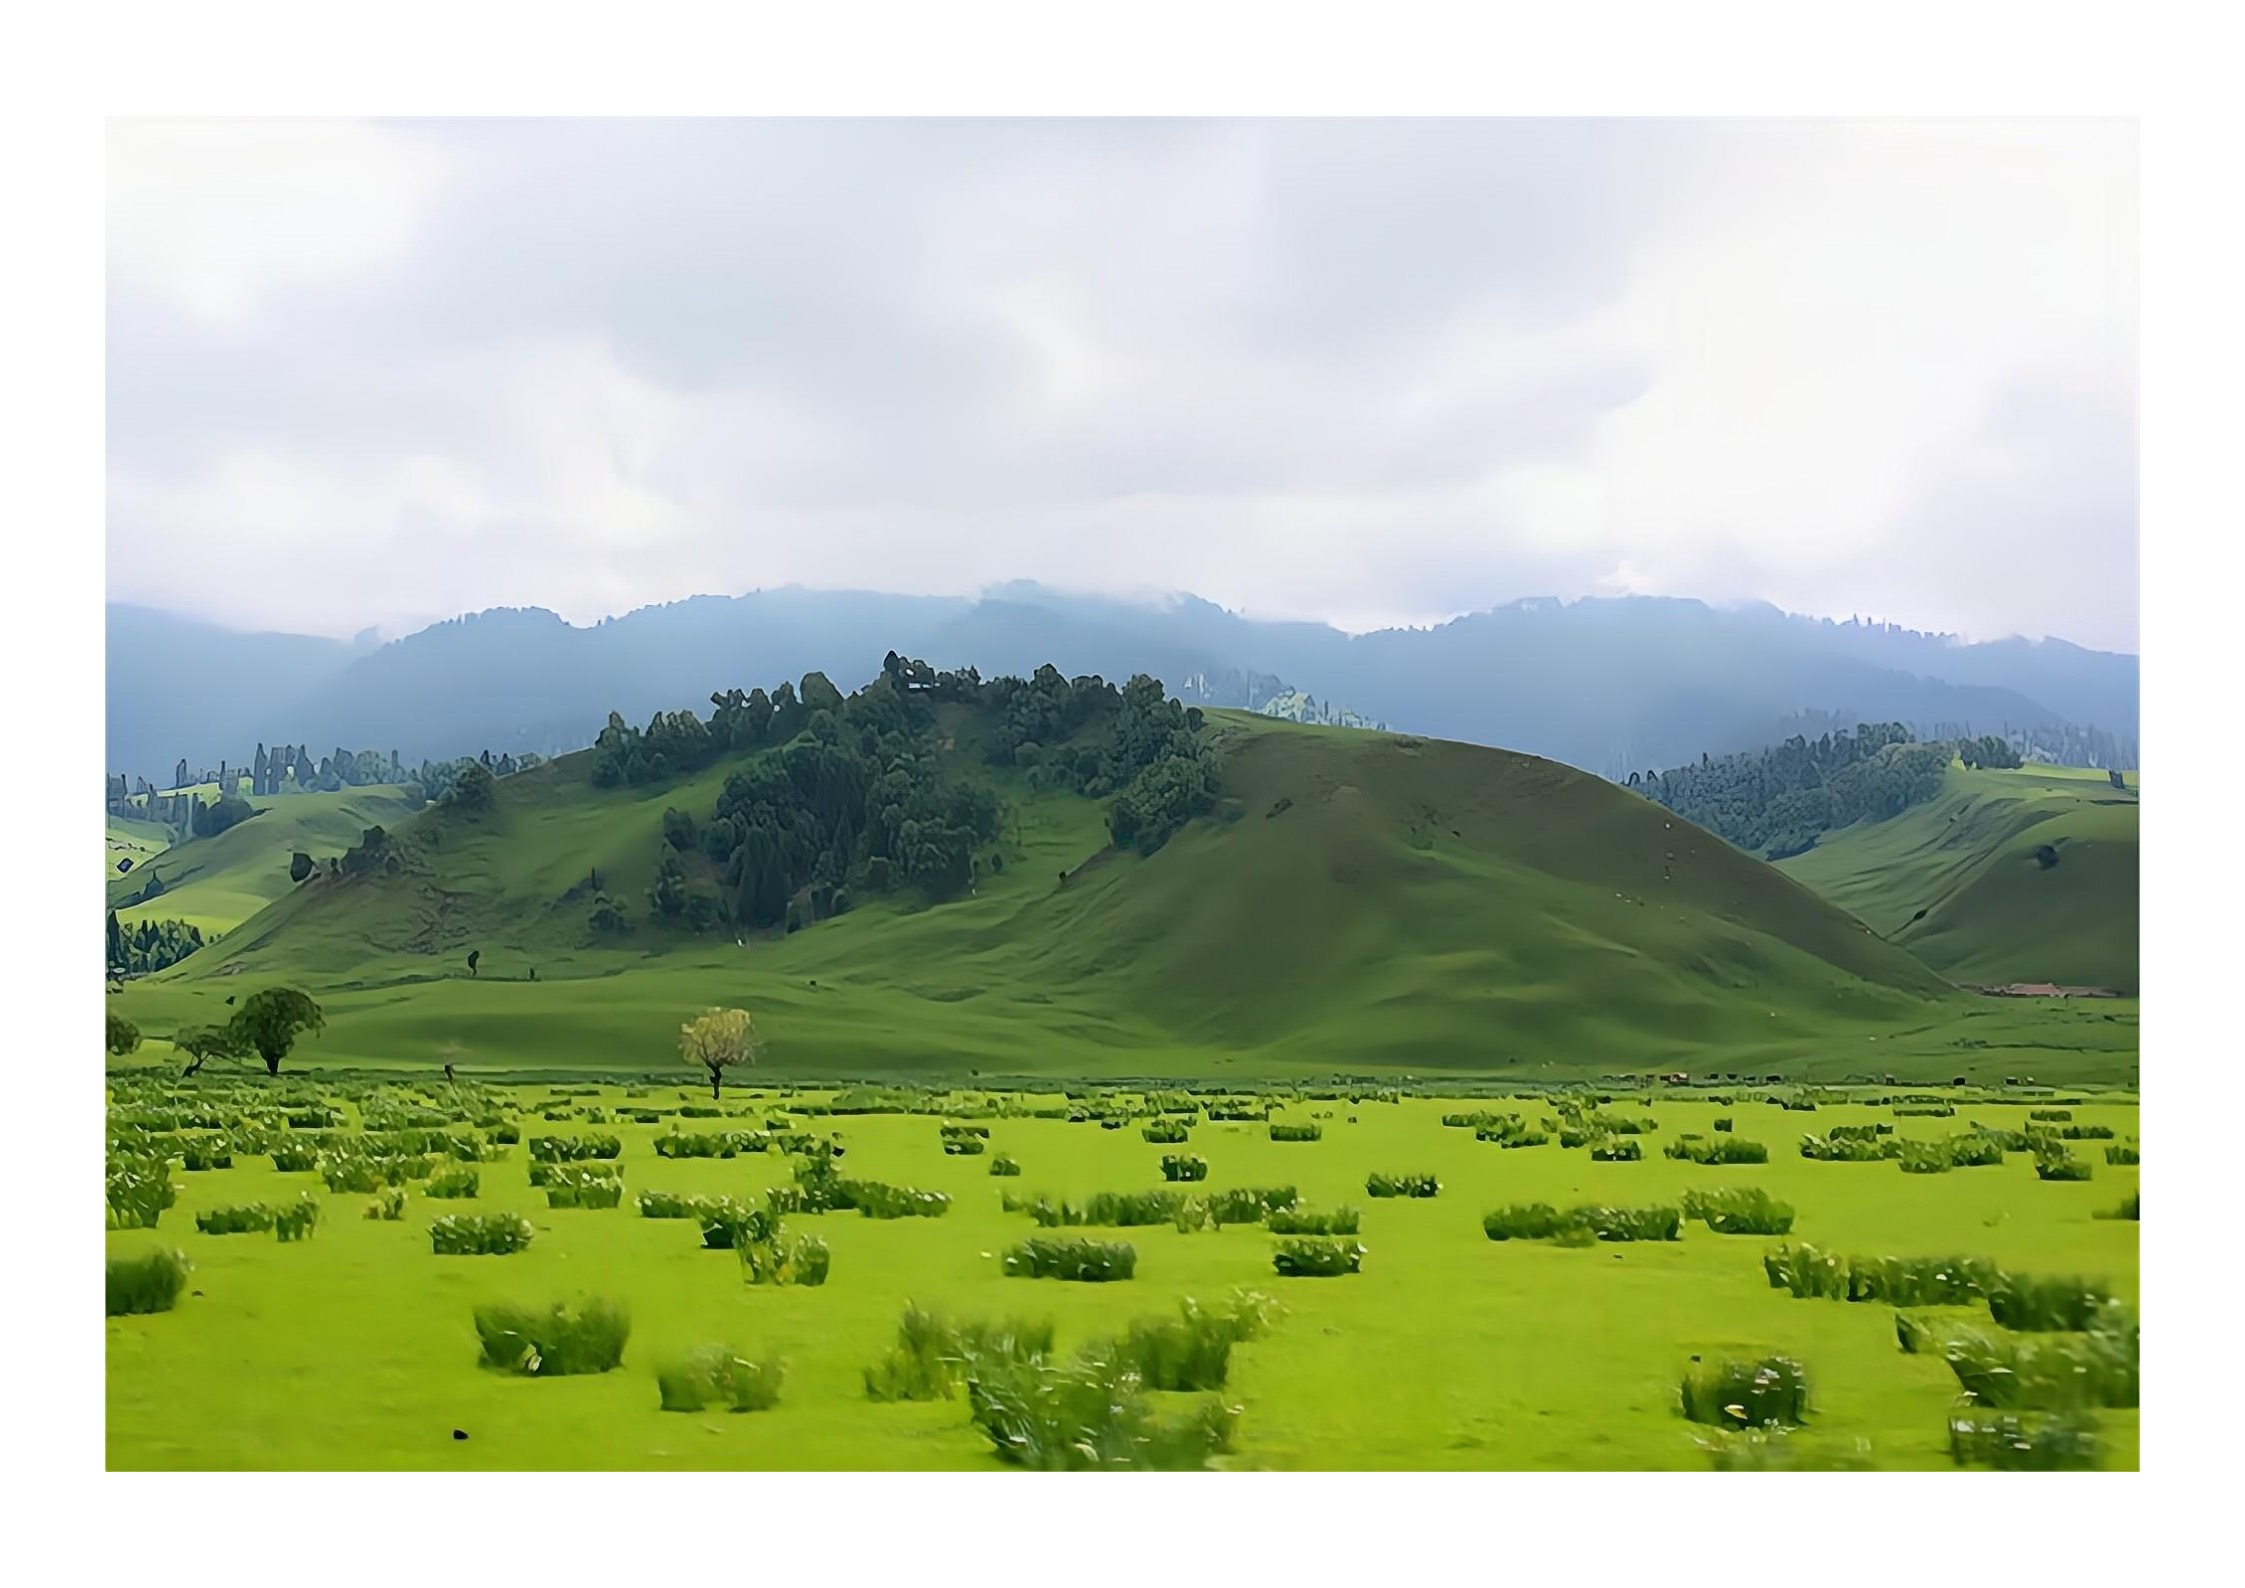
\includegraphics[width=1.05\textwidth]{./img/Fertile grassland.jpg}
\caption{Fertile grassland}
\end{subfigure}
\hfill
\begin{subfigure}[t]{0.48\textwidth}
\centering
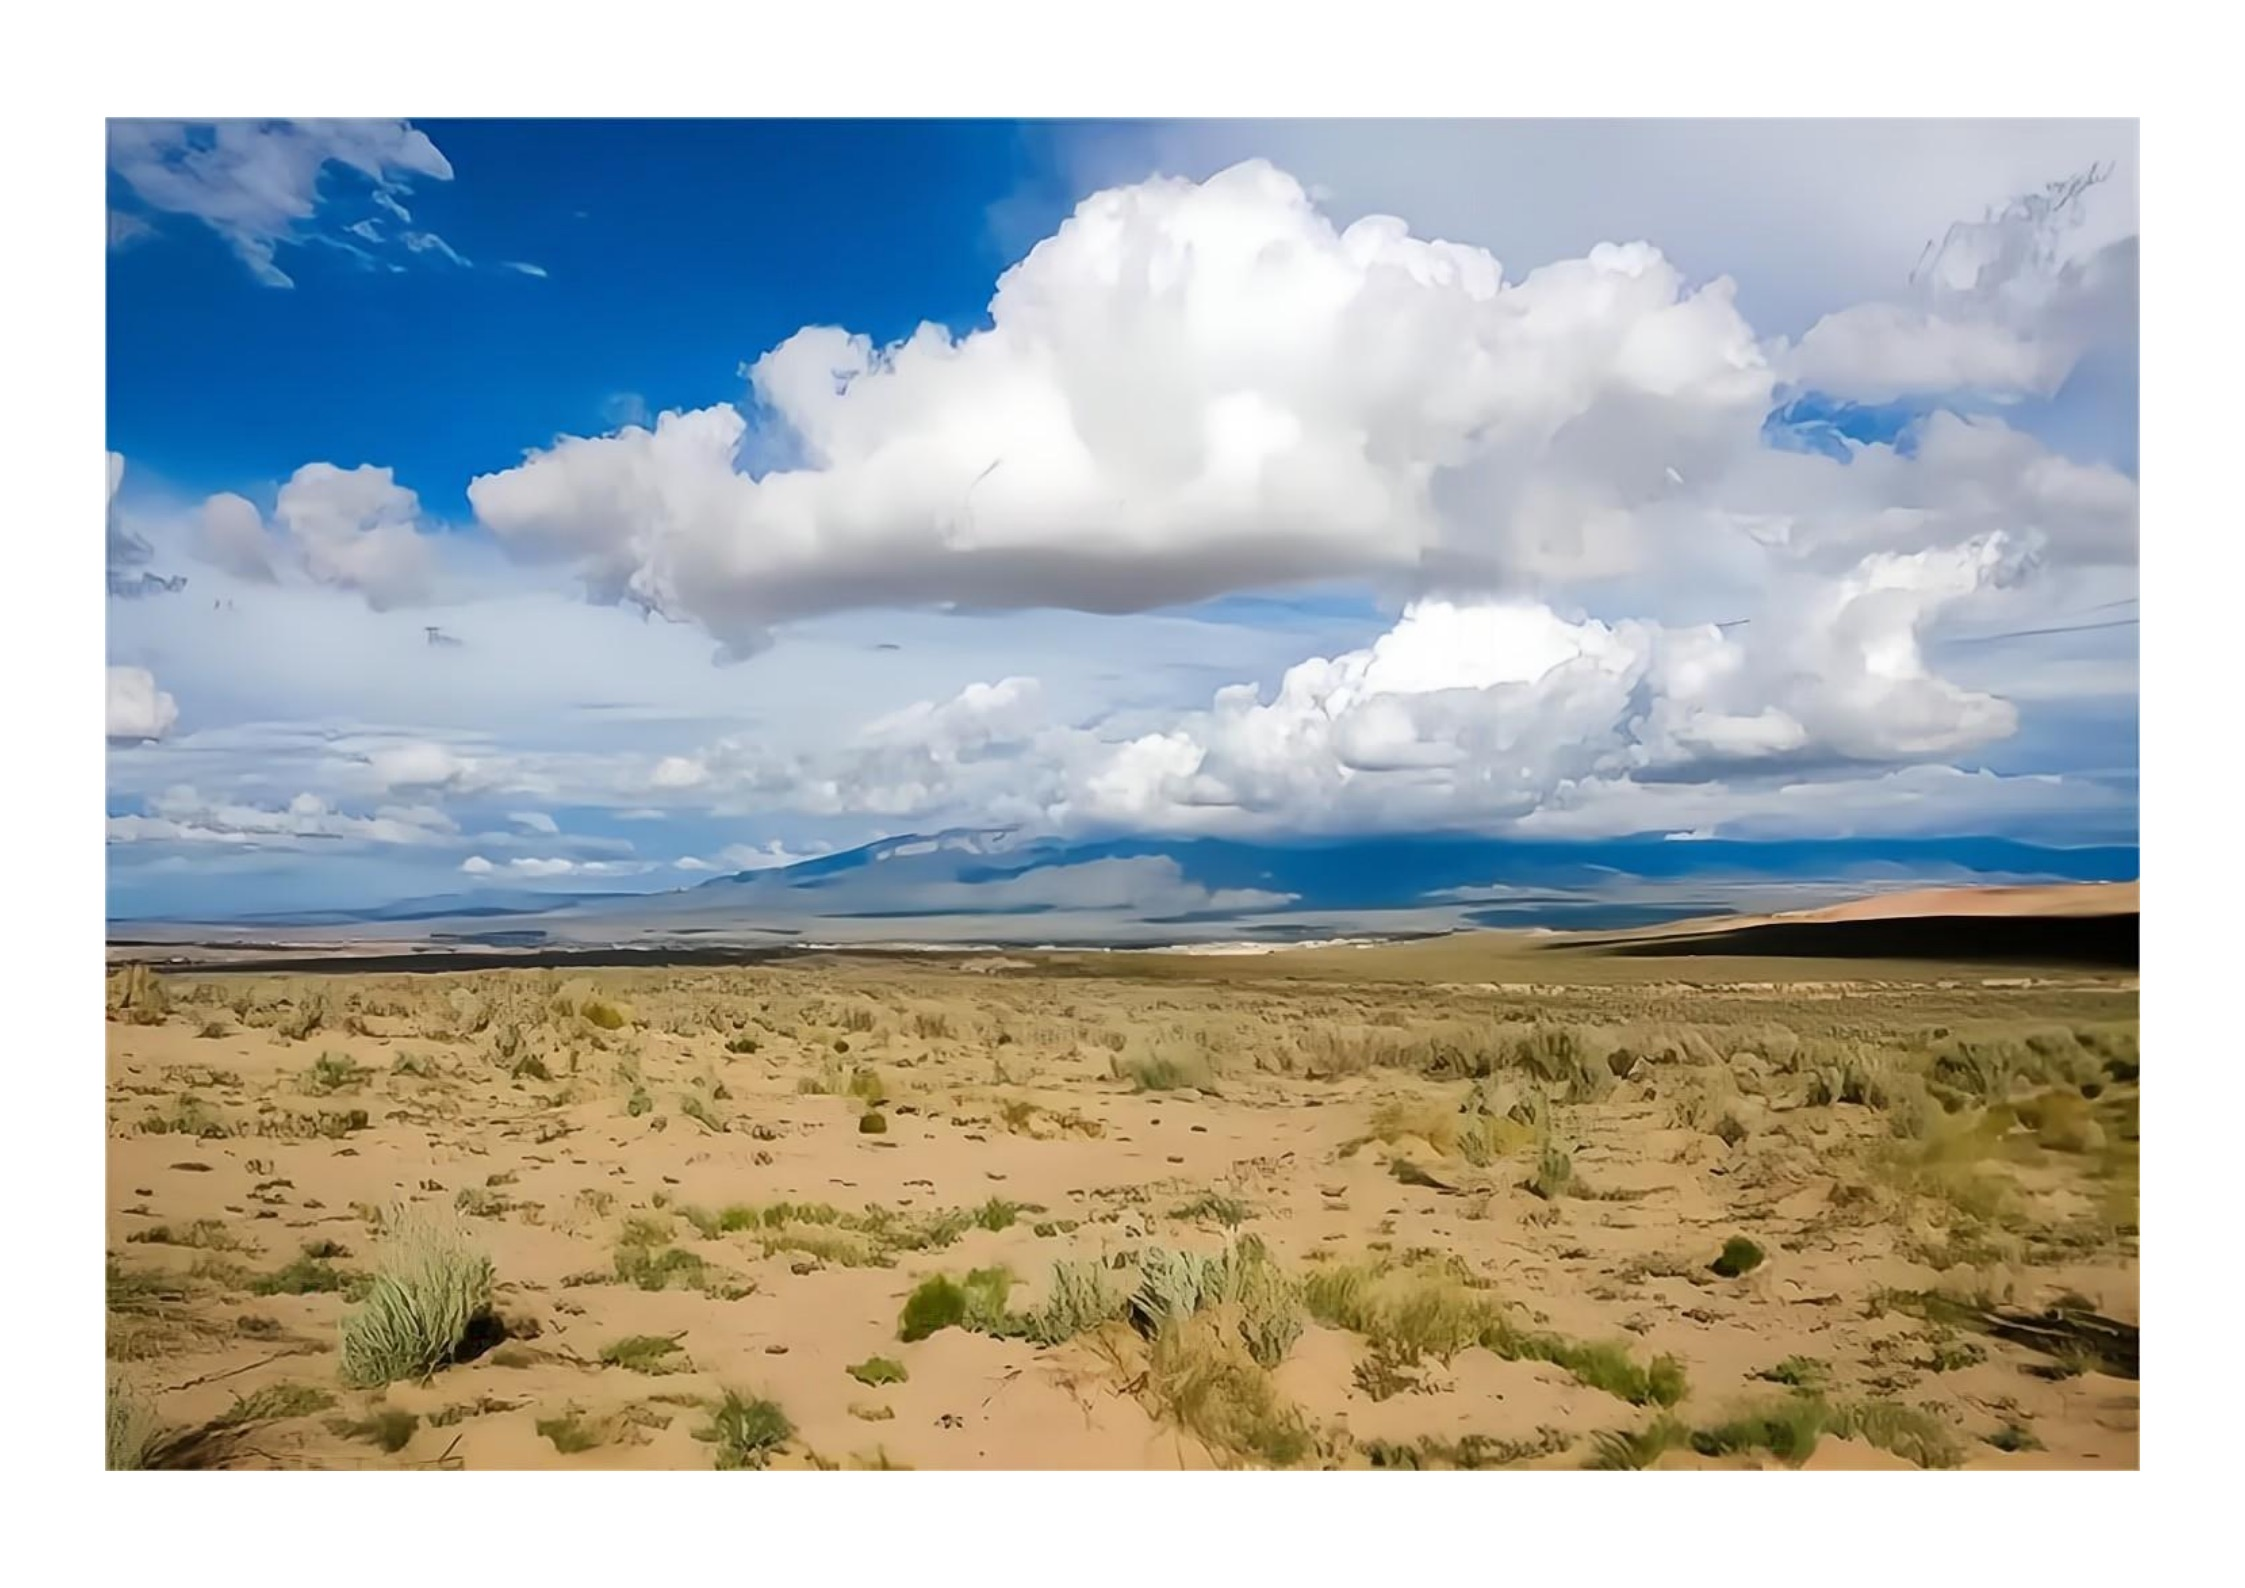
\includegraphics[width=1.05\textwidth]{./img/Barren grassland.jpg}
\caption{Barren grassland}
\end{subfigure}
\caption{Flora of the grassland \cite{1}}
\label{fig:grassland}
\end{figure}

\subsection{Restatement at the Problem}

\indent

Based on the background information and our understanding of the problem statement, the problems we need to address are as follows:

\begin{itemize}

\item Build a mathematical to predict the change of plant communities with a different number of species over time and derive the results under varying frequencies and levels of severity of droughts to see if there are differences. 

\item Consider the interactions between different species in the model and explains how different types of species can affect the outcome.

\item Analyze the relationship between a plant community's localized diversity and drought resistance to identify the minimum number of species that facilitate plant resistance to drought.

\item Use the model to illustrate how to ensure the long-term viability of a plant community and apply the model to a larger environment to see if the results change.

\item Identify how some environmental changes other than drought, such as pollution and habitat reduction, would affect the conclusions.


\end{itemize}

\subsection{Our Work}

\indent

In order to understand the relationship between drought adaptability and the number of species in the plant community, we conduct the following work:

\begin{itemize}
\item We collect \textbf{precipitation and temperature data} on a typical U.S. grassland region and select eight typical prairie plants with different attributes for study.

\item To study the intergenerational effects of plants, we develop \textbf{the Genotype Selection Model}, where we discuss the species' evolution trend.

\item To study the interspecific competition in plant communities, we develop \textbf{the Competition Model}. We use hierarchical analysis to calculate the weights of different plant attributes and derive the relative competitiveness of each plant.

\item To analyze the interaction between plants and their living environment, we build \textbf{the Interaction Model}. We focus on two environmental factors: precipitation and temperature, and use the Finite Elements Analysis (FEA) method to address this problem. From the resulting solutions, we plot the curves of biomass and soil moisture content over time as well as obtain the fertility factor for each generation.

\item To assess the model we build, we first introduce the \textbf{Shannon index} to measure the localized biodiversity. Then, we impose the effects of drought in the model and vary the frequency and severity of it in the presence of different numbers of plant species, so as to assess the relationship between the biodiversity and the community's drought adaptability.

\item Finally, to further test the reliability of our model, we change the habitat size, as well as impose the impact of pollution.

\end{itemize}

In general, we base the model construction on actual data and take various factors into consideration, such as interspecific competition, biotic and abiotic interactions, and different environmental conditions. The model is logical and hierarchical and has significant guidance for reality.

For a better understanding of the overall model, a flowchart is provided to describe the modeling process, as shown in Figure \hyperref[fig:model]{\textcolor{blue}{2}}.

\begin{figure}[h]
\centering
\begin{subfigure}{0.82 \textwidth}
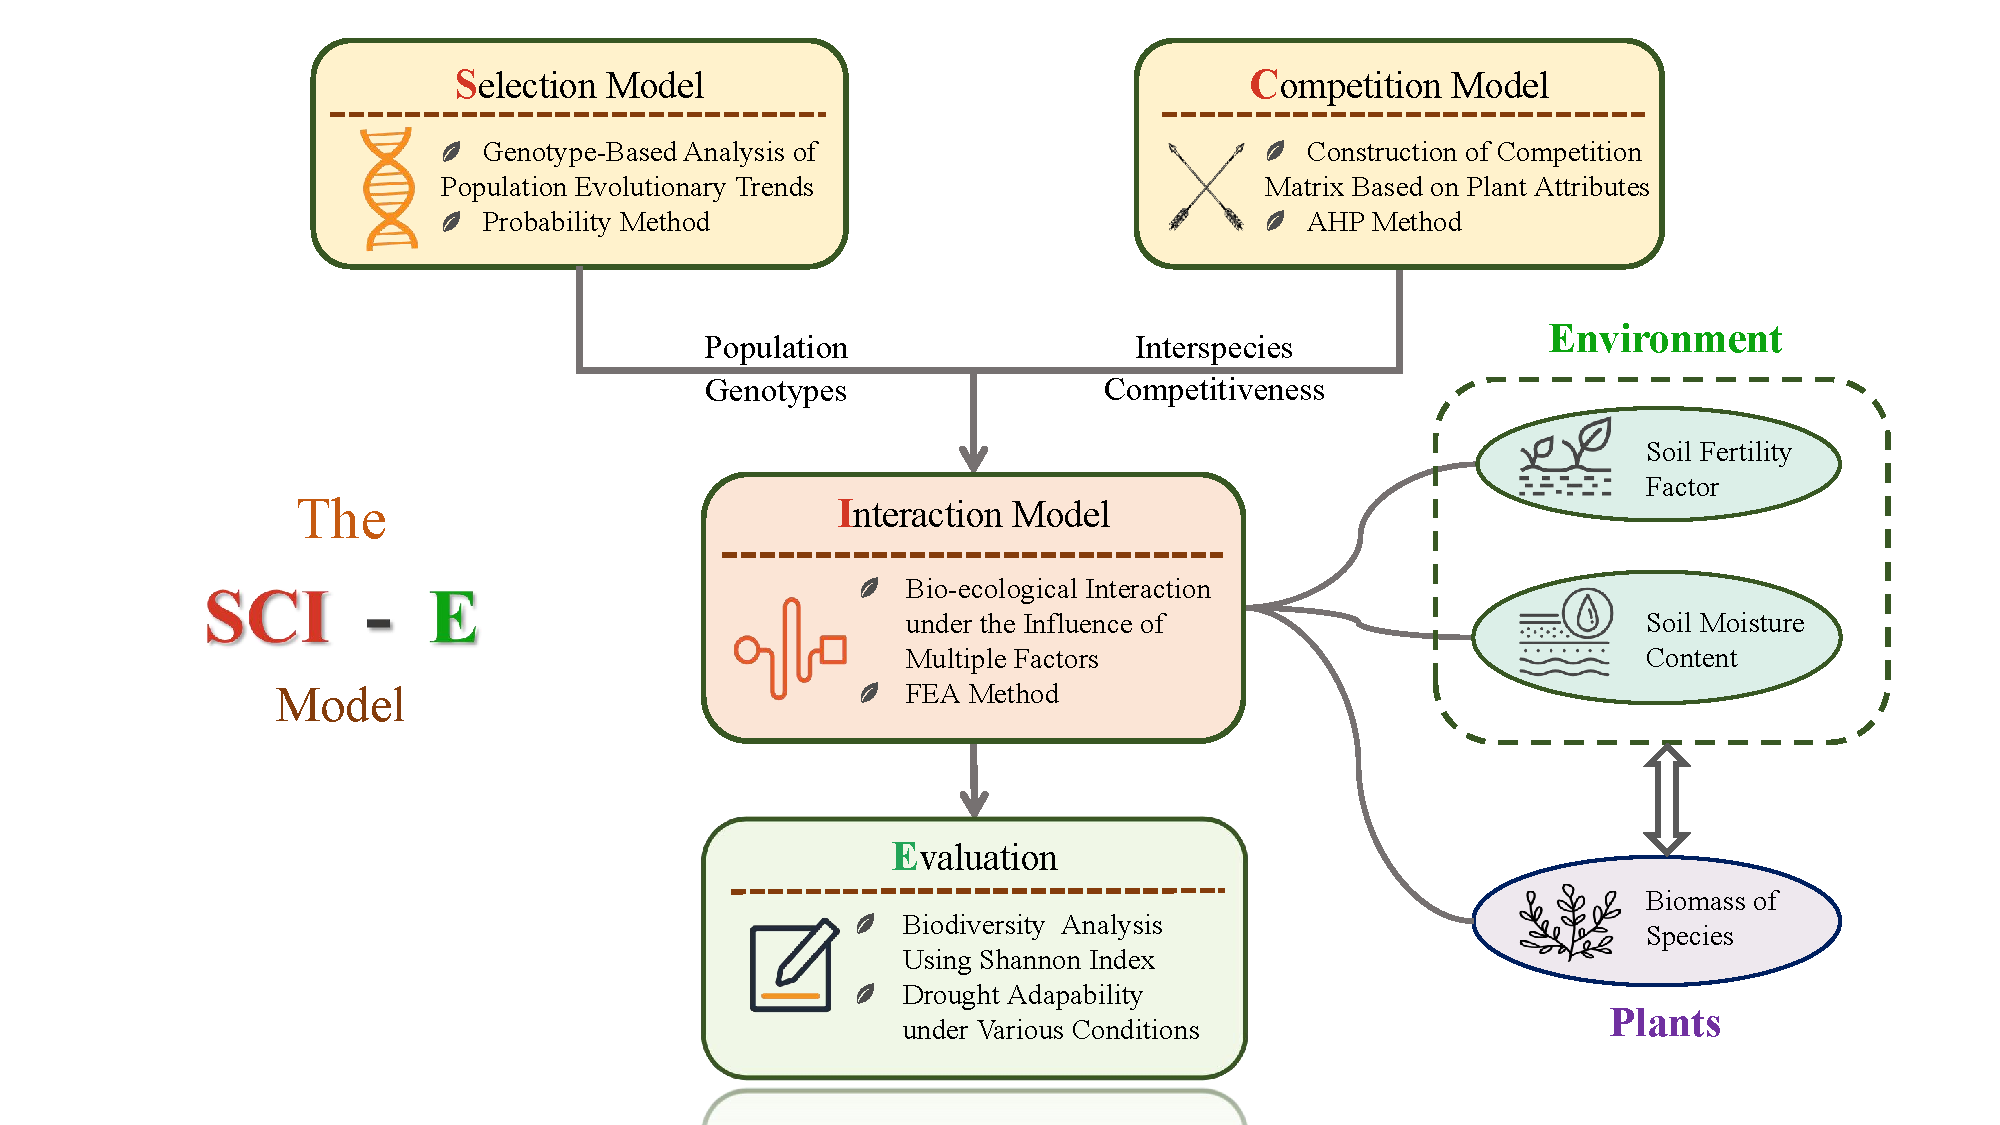
\includegraphics[width=\textwidth]{img/process.pdf}
\end{subfigure}
\caption{Model overview}
\label{fig:model}
\end{figure}

\section{Assumptions and Justification}

\indent

To simplify the problem, we make the following basic assumptions, each adequately justified.

\begin{itemize}
\item {\bf Assumption 1: Species migration in and out and genetic mutations are not considered. Mating between plants of the same species is random, and the hybridization of different species is not considered.}

{\bf Justification}: Here, we consider a relatively closed region with no species migration. In such an ideal environment, we assume that conspecifics mate randomly and do not interbreed.

\item {\bf Assumption 2: Environmental factors other than precipitation and temperature (e.g., light conditions, CO2 concentration in the air, etc.) are suitable and do not fluctuate greatly}

{\bf Justification}: Drought is a common environmental problem we care about. Therefore, we only consider the two environmental factors that are most closely related to it: precipitation and temperature. We assume that the other environmental factors affecting plant growth are suitable, do not fluctuate significantly, and set them to fixed values.

\item {\bf Assumption 3: Use the day's average temperature to represent the day's temperature.}

{\bf Justification}: Because we are concerned with the long-term evolution of plant communities in different environments, using the month as the unit of time, we can use the average temperature of the day to represent the temperature of a specific day.

\item {\bf Assumption 4: Disregard the impact of consumers on plants in the ecosystem.}

{\bf Justification}: Since the study focuses solely on the relationships and interactions between plants and other abiotic factors in the ecosystem, the influence of the consumers can be ignored when addressing the problem.

\item {\bf Assumption 5: Soil fertility for plants in each generation is influenced only by the previous generation, without considering the influence of earlier generations of plants.}

{\bf Justification}: We only focus on the direct effects of a single generation of plants on soil fertility while disregarding previous generations' indirect or legacy impact. In this case, we intentionally simplify the research design to exclude the influence of earlier plant generations on soil fertility. This assumption allows for a more focused analysis of the relationships between the current generation of plants and the soil they are growing.

\end{itemize}

\section{Notations and Definitions}

\indent

We begin by defining a list of notations(symbols) used in this article. We define the main parameters, while the specific value of those parameters will be given later.

\begin{table}[htbp]
\begin{center}
\caption{Notations in the SCI-E model}
\begin{tabular}{clc}
\toprule
{\bf Symbols} & {\bf Description} & \quad {\bf Unit} \\[0.1cm]
\midrule
$n$ & The number of plant population & \quad \SI{}{day} \\[0.1cm]
$t$ & The time from now  & \quad \SI{}{day} \\[0.1cm]
$C(t)$ & Soil moisture content & \quad / \\[0.1cm]
$P(t)$ & Precipitation rate & \quad \SI{}{\cubic\meter \cdot day^{-1}} \\[0.1cm]
$E(t)$ & Evaporation rate & \quad \SI{}{\cubic\meter \cdot day^{-1}} \\[0.1cm]
$e_i$ & Evaporation rate per unit of plant biomass of the \textit{i}-th species & \quad \SI{}{m^5\cdot day^{-1}} \\[0.1cm]
$f(m)$ & The soil fertility factor of the \textit{m}-th generation & \quad \SI{}{m^{-3}} \\[0.1cm]
$f_0$ & The initial soil fertility factor & \quad \SI{}{m^{-3}} \\[0.1cm]
$K(t)$ & Environmental capacity & \quad \SI{}{m^{-2}} \\[0.1cm]
$d$ & Density of the \textit{i}-th plant & \quad \SI{}{m^{-2}} \\[0.1cm]
$T_0$ & Initial temperature & \quad $^\circ \mathrm{F}$ \\[0.1cm]
$T_e$ & Present temperature & \quad $^\circ \mathrm{F}$ \\[0.1cm]
$\alpha_{i,j}(t)$ & Relative competitiveness of species $i$ to species $j$ & \quad / \\[0.1cm]
$a_i$ & Water absorption capacity of the \textit{i}-th species  & \quad / \\[0.1cm]
$r_i$ & Reproductive capacity of the \textit{i}-th species  & \quad / \\[0.1cm]
$v_i$ & Viability of the \textit{i}-th species  & \quad / \\[0.1cm]
$m_i(t)$ & Biomass of the \textit{i}-th species   & \quad  \SI{}{\gram\cdot \meter^{-2}} \\[0.1cm]
$c_{i}$ & Optimum moisture content of the \textit{i}-th species  & \quad /  \\[0.1cm]
$g_{i,k}$ & The frequency of the \textit{k}-th genotype of the \textit{i}-th species   & \quad  / \\[0.1cm]
\bottomrule
\end{tabular}
\end{center}
\label{tab:notations}
\end{table}

\section{Data Preparation}

\subsection{Plants}

\indent

Plants on the grassland often face the threat of drought. These plants usually have strong adaptation capabilities and can grow in dry and hot conditions. 

To study the drought adaptability of different plant species while considering intergenerational effects, we focus on the three attributes of plants: water absorption ability, reproductive capacity, and viability. The water absorption ability directly affects a plant's utilization of water in a dry environment; The reproductive capacity is a critical factor in maintaining the survival and expansion of a population; The survival ability affects the survival of individuals in unsuitable environments as well as the continuity of populations.

We select $8$ typical plants on the American prairie for our study, including \textit{Tea Arthropod, Airplane Grass, Galangal, Lemongrass, Eupatorium Odoratum, Persicaria Chinensis, Purple Alfalfa, }and \textit{Horseshoe Grass}. They differ from each other in these three attributes. For example, Tea Arthropod is a desert plant that can survive in poor soil and water-deficient conditions, while Galangal can grow in hot and dry environments.

\begin{figure}[htbp]
\centering
\begin{subfigure}[t]{0.48\textwidth}
\centering
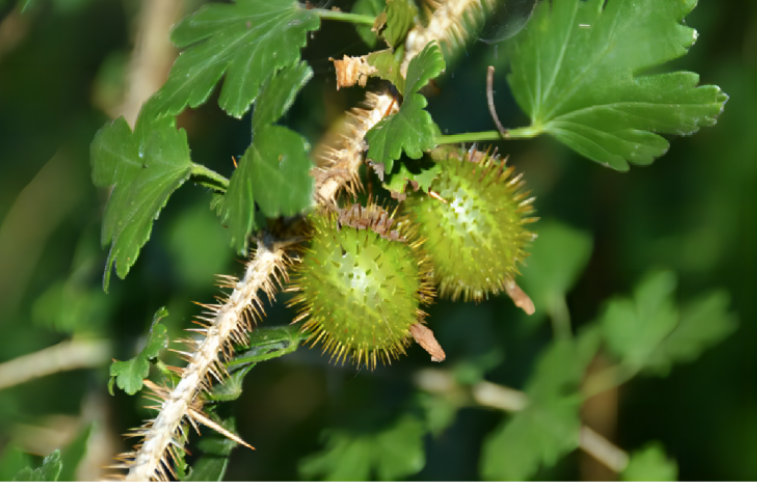
\includegraphics[width=0.85\textwidth]{./img/Tea Arthropod.png}
\caption{Tea Arthropod}
\end{subfigure}
\hfill
\begin{subfigure}[t]{0.48\textwidth}
\centering
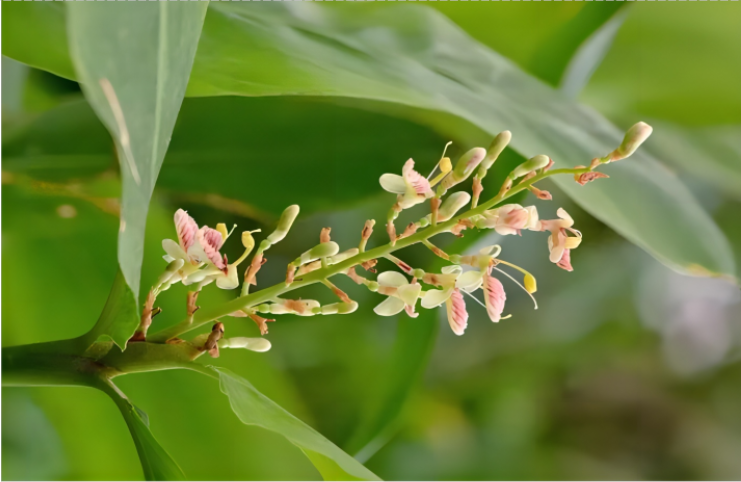
\includegraphics[width=0.85\textwidth]{./img/Galangal.png}
\caption{Galangal}
\end{subfigure}
\caption{Two typical grassland plants \cite{1}}
\end{figure}

\subsection{Weather}

\indent

We retrieve the monthly precipitation and temperature data of New Mexico, a prairie region in the United States, from 1894 on the website of the National Weather Service \cite{2}. Through preliminary drawing and observation in excel, we find that the precipitation showed a clear cyclical rule with the change of months. 

Therefore, we conduct \textbf{Fourier analysis} on the precipitation data from 1990 to 2000. The formula of precipitation variation with month is obtained, and we take this formula as the basic model of $P(t)$. We analyze the temperature similarly and obtain the temperature change mode $T_e(t)$ over time. Two plots are shown in Figure \hyperref[fig:weather]{\textcolor{blue}{4}}.


\begin{figure}[htbp]
\centering
\begin{subfigure}[t]{0.48\textwidth}
\centering
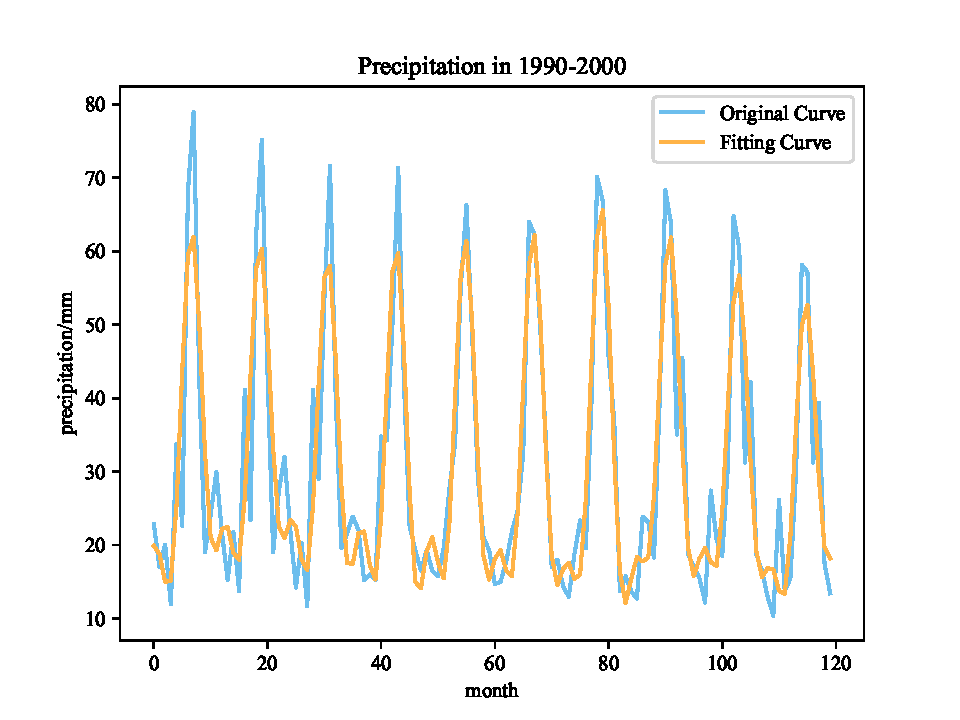
\includegraphics[width=0.9\textwidth]{img/precipitation in 1990-2000.pdf}
\caption{Precipitation}
\end{subfigure}
\hfill
\begin{subfigure}[t]{0.48\textwidth}
\centering
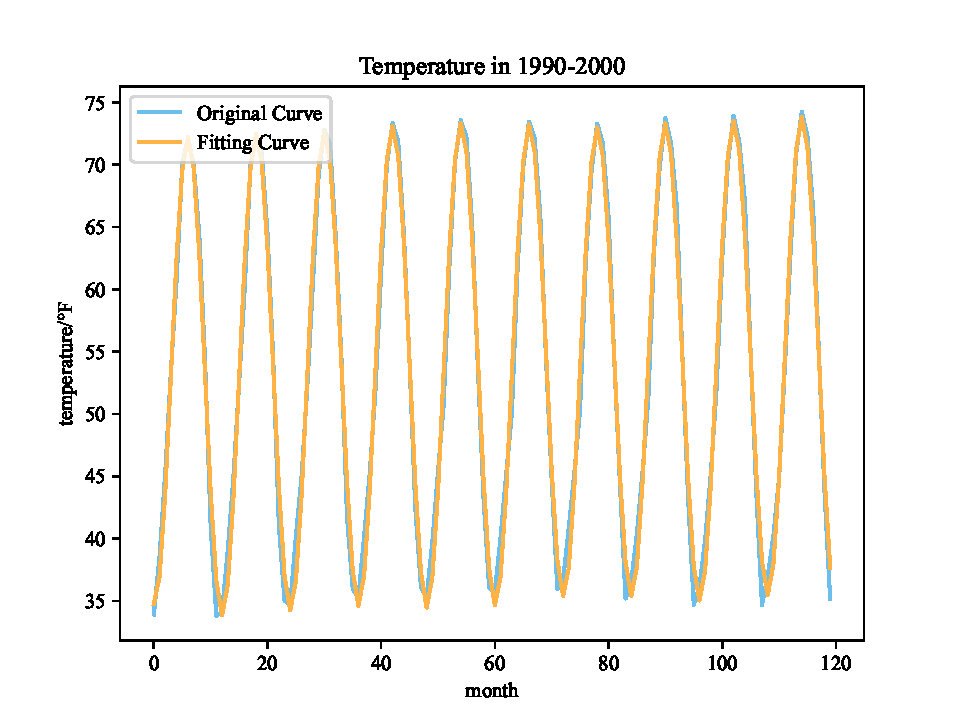
\includegraphics[width=0.9\textwidth]{img/temperature in 1990-2000.pdf}
\caption{Temperature}
\end{subfigure}
\caption{Weather in New Mexico from 1990 to 2000}
\label{fig:weather}
\end{figure}



\section{The SCI-E Model}

\subsection{Selection Model: Long-Term Genotype Selection Model}

\subsubsection{Model Design}

\indent

We use $\mathcal{G}_i$ for the set of all genotypes of the \textit{i}-th species and $\mathcal{K}_i$ for the set of all drought-resistant genotypes of the \textit{i}-th species. Assume that all plant populations are diploid. For plant $i$, the dominant alleles associated with drought resistance are $\mathrm{B}_1, \mathrm{B}_2, \cdots \mathrm{B}_l$, where the number of all the genotypes related to drought resistance is $l$. 

Therefore, all the genotypes and the genotypes associated with drought adaptation are as follows: $\mathcal{G}  =\left\{\mathrm{B}_k \mathrm{~B}_k, \mathrm{~B}_k \mathrm{~b}_k, \mathrm{~b}_k \mathrm{~b}_k \mid k=1, \cdots, l\right\}$, $\mathcal{K}  =\left\{\mathrm{B}_k \mathrm{~B}_k, \mathrm{~B}_k \mathrm{~b}_k \mid k=1, \cdots, l\right\}$, where one generation later, $\mathrm{b}_{\mathrm{i}} \mathrm{b}_{\mathrm{i}}$ in the dominant gene dies due to the irregular drought. Assume that the ratio of $\mathrm{B}_i \mathrm{B}_i, \mathrm{B}_i \mathrm{b}_i, \mathrm{b}_i \mathrm{b}_i$ in the initial state is $\eta_{i 1}, \eta_{i 2}, \eta_{i 3}$, and  then the proportion of each allele in the mating is

\begin{equation}
\mathrm{B}_k: \mathrm{b}_k=\eta_{k 1}+\frac{1}{2} \eta_{k 2}: \frac{1}{2} \eta_{k 2} \quad k=1, \cdots, d
\end{equation}

Whether each dominant allele is expressed in the offspring can be viewed as a binomial distribution $X_k \sim B\left(1, p_k\right)$, where:

\begin{equation}
p_k=\frac{2 \eta_{k 1}+\eta_{k 2}}{2\left(\eta_{k 1}+\eta_{k 2}\right)} \quad k=1, \cdots, d
\end{equation}

Then the proportion of the three genotypes $\mathrm{B}_i \mathrm{B}_i, \mathrm{B}_i \mathrm{b}_i, \mathrm{b}_i \mathrm{b}_i$ in the offspring will be as follows:

\begin{equation}
\eta_{i 1}^{\prime}=p_i^2, \eta_{i 2}^{\prime}=2 p_i\left(1-p_i\right), \eta_{i 3}^{\prime}=\left(1-p_i\right)^2
\end{equation}

\subsubsection{Data Simulation}

\indent

For calculation convenience, we assume that $d=2$ and the initial proportion of drought-resistant homozygote, drought-resistant heterozygote, and non-drought resistant homozygote is $1: 1: 1$. Assume that when the population reaches stability, it follows a normal distribution:

$$
N_1\left(K, \sigma_1^2\right), K=1000, \sigma_1=100
$$

On the other hand, to better simulate the real grassland situation, Gaussian noise is introduced to the binomial distribution in the reproduction process, which is also assumed to satisfy a normal distribution:

$$
N_2\left(p, \sigma_2^2\right), \sigma_2=0.01
$$

The trend of the proportion of drought resistance traits simulated by the model over time is shown in Figure \hyperref[fig:gene]{\textcolor{blue}{5}}:

\begin{figure}[h]
\centering
\begin{subfigure}{0.55 \textwidth}
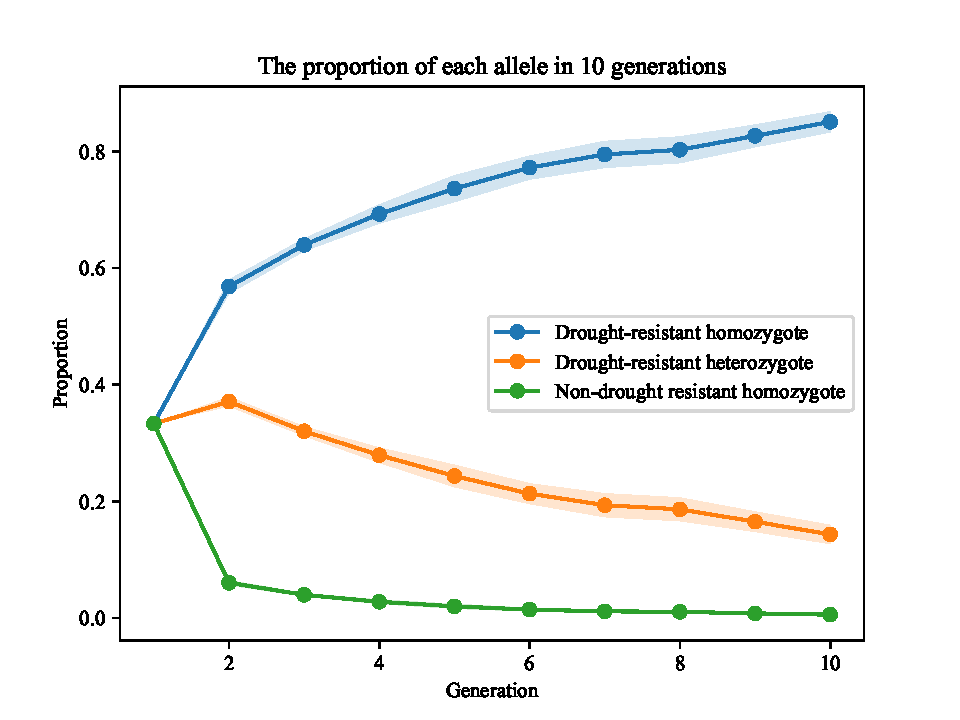
\includegraphics[width=1\textwidth]{img/The proportion of each allele in 10 generations.pdf}
\end{subfigure}
\caption{The proportion of each allele in 10 generations}
\label{fig:gene}
\end{figure}

The graph shows that the proportion of drought-tolerant purest in each plant population gradually increases, representing the process of \textbf{Natural Selection}.

\subsection{Competition Model: Interspecific Competition Model Based on AHP}

\subsubsection{Data Collection}

\indent

We search some essays about the plants we choose, which discuss
Those plants ' reproductive capacity and water absorption ability through growing experiments and field surveys. According to references \cite{3}\cite{4}, we search for information about $8$ representative plants and score their viabilities, reproductive capacities, and water absorption capacities. The results are listed in Tabel \hyperref[tab:Evaluation]{\textcolor{blue}{2}}. To visualize the properties of various plants, we plot the results on a radar map, as shown in Figure  \hyperref[fig:radar]{\textcolor{blue}{6}}.

\begin{table}[htbp]
\caption{Evaluation of viabilities, reproduction capacities, and water absorption capacities}
\centering
\begin{tabular}{@{}cccc@{}}
\toprule
Plant Name & $v_i$ & $r_i$ & $a_i$ \\
\midrule
Tea Arthropod & 7.3 & 5.2 & 11.1 \\
Airplane Grass & 1.7 & 4.3 & 11.0 \\
Galangal & 3.8 & 3.4 & 10.3 \\
Lemongrass & 3.4 & 4.6 & 9.3 \\
Eupatorium odoratum & 7.4 & 7.5 & 7.8 \\
Persicaria chinensis & 5.4 & 7.2 & 7.3 \\
Purple Alfalfa & 6.3 & 7.2 & 5.6 \\
Horseshoe grass & 10.6 & 10.8 & 4.2 \\
\bottomrule
\label{tab:Evaluation}
\end{tabular}
\end{table}

\begin{figure}[h]
\centering
\begin{subfigure}{0.42 \textwidth}
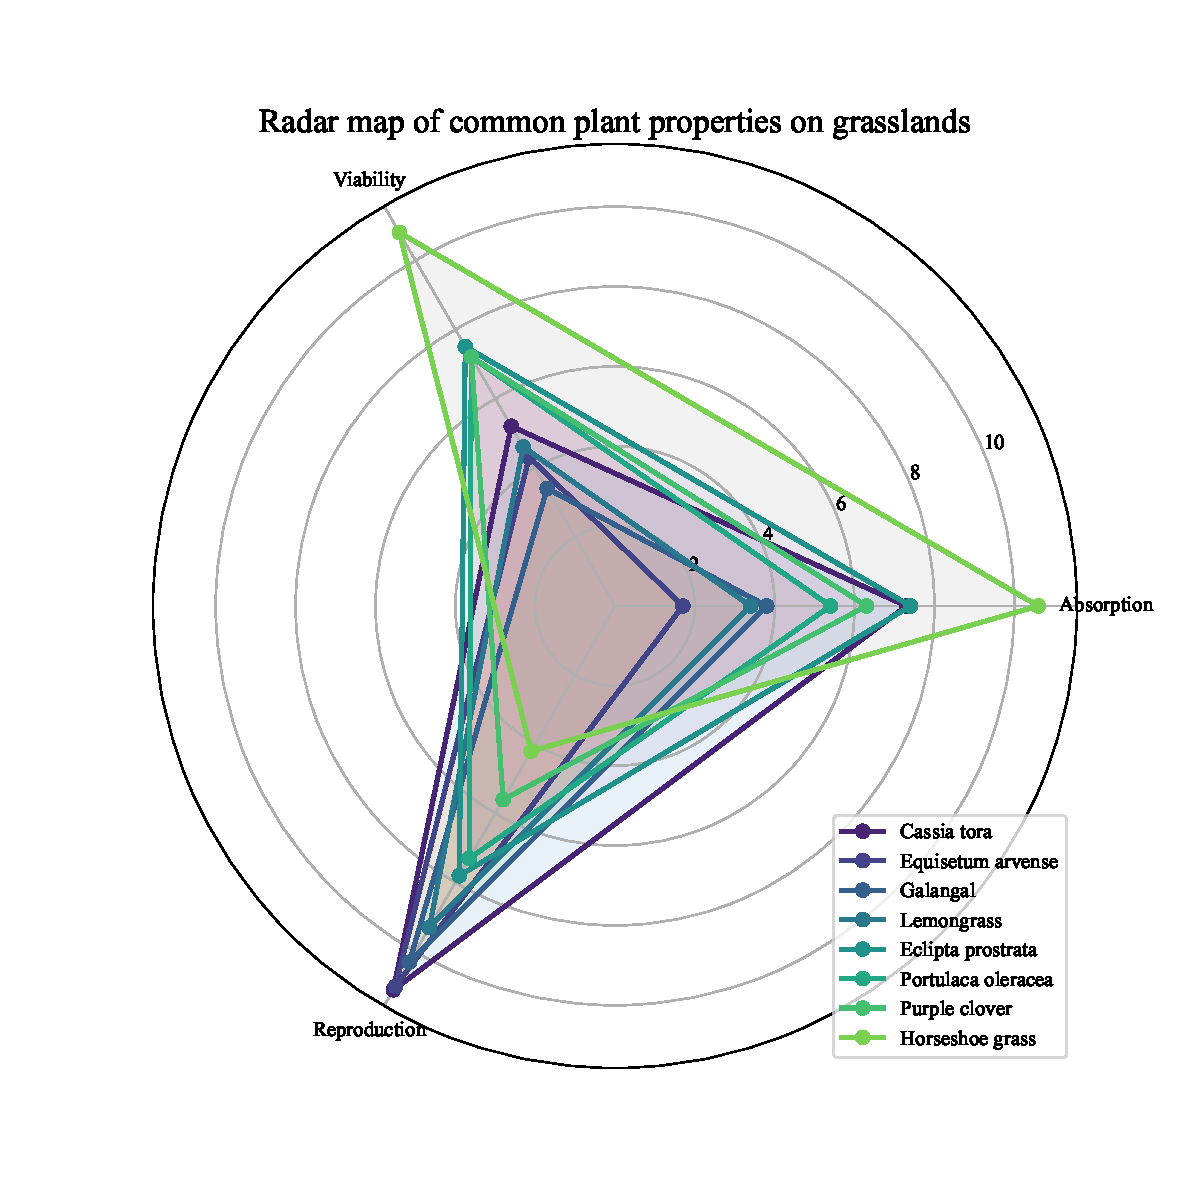
\includegraphics[width=1\textwidth]{img/Radar map of common plant properties on grasslands.pdf}
\end{subfigure}
\caption{Radar map of common plant properties on grasslands}
\label{fig:radar}
\end{figure}


\subsubsection{Determining the Weight of the Three Factors }

\indent

Using Analytic Hierarchy Process (AHP), we obtain the weights of these three factors for the interspecific competitiveness of plants. The specific process is as follows: 

Firstly, we derive the weight matrix between the above three factors based on biological studies \cite{5}, as shown in Table  \hyperref[tab:comparison matrix]{\textcolor{blue}{3}}.

\begin{table}[htbp]
  \centering
  \caption{The comparison matrix of three plant factors}
  \begin{blockarray}{cccc}
& \text{$v_i$} & \text{$r_i$} & \text{$a_i$} \\
\begin{block}{c[ccc]}
$v_i$ & 1.000 & 0.333 & 0.143   \\
$r_i$ & 3.000 & 1.000 & 0.333   \\
$a_i$ & 7.000 & 3.000 & 1.000  \\
\end{block}
\end{blockarray}
    \label{tab:comparison matrix}
\end{table}


From this matrix, we calculate the consistency ratio $C R=\dfrac{C l}{R I}=0.012<0.1$, which passes the consistency check.
Thus we obtain the final relative weights of the three factors:

\begin{table}[htbp]
\centering
\caption{Final relative weights of three plant factors}
\begin{tabular}{ccc}
\toprule
Viability & Reproductive Capacity & Water Absorption Capacity \\
\midrule
0.0879 & 0.2426 & 0.6694 \\
\bottomrule
\end{tabular}
\label{tab:weights}
\end{table}

\subsubsection{Determine the Competition Matrix between Species}

\indent

Based on the weights of the $3$ factors, we obtain the final scores of the eight species under AHP:

\begin{table}[ht]
\centering
\caption{Total plant attribute score under AHP method}
\label{tab:plants}
\begin{tabular}{ccccc}
\toprule
Plant Name & $v_i$ & $r_i$ & $a_i$ & Total Score / Label \\
\midrule
Tea Arthropod & 7.3 & 5.2 & 11.1 & 15.40 / 0 \\
Airplane Grass & 1.7 & 4.3 & 11.0 & 10.09 / 1 \\
Galangal & 3.8 & 3.4 & 10.3 & 10.94 / 2 \\
Lemongrass & 3.4 & 4.6 & 9.3 & 9.87 / 3 \\
Eupatorium odoratum & 7.4 & 7.5 & 7.8 & 13.45 / 4 \\
Persicaria chinensis & 5.4 & 7.2 & 7.3 & 11.66 / 5 \\
Purple Alfalfa & 6.3 & 7.2 & 5.6 & 10.31 / 6 \\
Horseshoe grass & 10.6 & 10.8 & 4.2 & 16.14 / 7 \\
\bottomrule
\end{tabular}
\label{tab:score}
\end{table}

The $8$ plants are labeled $0,1, \ldots, 7$, in the order shown in Table  \hyperref[tab:score]{\textcolor{blue}{5}}. We define the relative competition factor of species $i$ for species $j$ as $\alpha_{i j}$, which is the ratio of the total scores of species $i$ to species $j$. Then we obtain a competition matrix for the eight species. We plot it on a heat map:

\begin{figure}[h]
\centering
\begin{subfigure}{0.548 \textwidth}
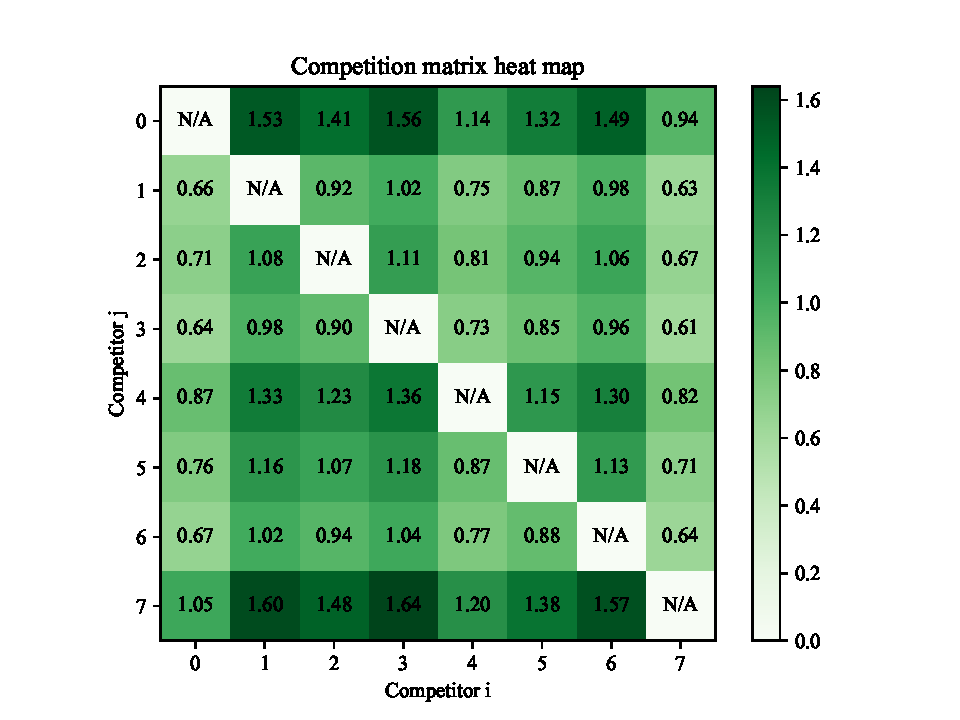
\includegraphics[width=1\textwidth]{img/competition matrix heat map}
\end{subfigure}
\caption{Competition matrix heat map}
\label{fig:heat}
\end{figure}

\subsection{Interaction Model: Multi-species Competition Model Based on FEA}

\subsubsection{Analysis and Modeling of Soil Moisture Content}

\indent

The change of soil moisture content $C(t)$ is proportional to the amount of precipitation minus the amount of evaporation and the amount of water absorbed by plants. Meanwhile, by reviewing the literature, we know that the soil water retention capacity is positively related to soil fertility, so within the scope of our model, they can be considered linearly related \cite{6}. Thus we can obtain the Equation below.

\begin{equation}
\frac{\mathrm{d} C(t)}{\mathrm{d} t}=(P(t)-E(t)) \cdot f(n)
\end{equation}

For water evaporation $E(t)$, it should be positively correlated with the current temperature according to Newton's Law of Cooling. Also, in aird areas, more local organisms can reduce the evaporation of soil moisture content \cite{7}, so we can obtain the equation below. Since the local annual temperature does not vary much, the change in water evaporation is not the main factor leading to drought.

\begin{equation}
E(t)=A\left(T_e(t)-T_0\right)-\sum_{i} e_i m_i(t)
\end{equation}

For the precipitation $P(t)$, on the one hand, in average years with non-drought conditions, we use the precipitation variation curve fitted by the actual data above. On the other hand, by looking at the historical data, we find that in the 1970s, when New Mexico experienced a drought, its annual precipitation was significantly lower than in average years. Therefore, in our model, we simulate drought conditions by adjusting the precipitation for that year to about $90 \%$ of the average value.


\subsubsection{Analysis and Modeling of Population Behavior in Grassland Communities}

\indent

\textit{The logistic equation} is the classical model in biology that describes the change in the number of individual populations. However, since the model describes the environmental accommodation of the purely external environment, we need to subtract a correction term for interspecific competition. This results in the modified logistic equation.

\begin{equation}
\frac{\mathrm{d} N(t)}{\mathrm{d} t}=r N(t)\left(1-\frac{N(t)}{K}\right) \Longrightarrow
\frac{\mathrm{d} m_i(t)}{\mathrm{d} t}=r_i m_i(t)\left(1-\frac{m_i(t)}{K_i(t)}\right)-\sum_{j \neq i} a_{j i} m_i(t) m_j(t)
\end{equation}

As an ecological article \cite{8} shows, the effect of soil moisture content on the efflux of CO$_2$ from soils has been described by the linear function of soil water expressed as water holding capacity, water-filled pore space, precipitation indices, and depth to the water table. The amount of CO$_2$ in the soil directly affects the environmental organisms' tendency to increase and decrease around the optimum environment, so we use the following h function to describe this trend.

\begin{equation}
h(x)=\left(-\left(x-c_0\right)^2+c_1\right) d
\end{equation}

Since the adaptability of plants to the environment is directly related to moisture content, the quadratic function of moisture content is multiplied by the frequency of surviving genes to evaluate the environmental tolerance at the current moisture content.

\begin{equation}
K_i(t)=h(C(t)) \cdot \sum_{k \in \mathcal{K}} g_{i k}
\end{equation}

Since the growth cycle of plants on the savannah tends to be one year, we analyze the changes in soil fertility every year. This year's grassland remains greatly improved soil fertility, so this year's index of soil fertility should equal the previous year's fertility plus the correction for this year's remains. Thus, the formula below is obtained.

\begin{equation}
f(n)=\lambda \sum_i m_i(n T)+f_0
\end{equation}


The differential equations mentioned above are organized according to environment and plant classification as follows:

$$
\mathrm{Differential\ equations}
\begin{cases}
\begin{aligned}  
&\mathrm{Environment}
\begin{cases}
\begin{aligned}
&\dfrac{\mathrm{d}\textcolor{blue}{C(t)}}{\mathrm{d} t}=(P(t)-E(t))\cdot \textcolor[rgb]{0.4, 0.26, 0.13}{f(n)} \\
&E(t)=A\left(T_e(t)-T_0\right)-\displaystyle\sum_i e_i \textcolor[rgb]{0.282, 0.561, 0.412}{m_i(t)} \\ 
\end{aligned} 
\end{cases}\\
&\mathrm{Plants}
\begin{cases}
\begin{aligned} 
&\dfrac{\mathrm{d} \textcolor[rgb]{0.282, 0.561, 0.412}{m_i(t)}}{\mathrm{d} t}=r_i \textcolor[rgb]{0.282, 0.561, 0.412}{m_i(t)}\left(1-\dfrac{\textcolor[rgb]{0.282, 0.561, 0.412}{m_i(t)}}{K_i(t)}\right)-\displaystyle\sum_{j\neq i} \alpha_{j i} \textcolor[rgb]{0.282, 0.561, 0.412}{m_i(t)}m_j(t) \\ 
&h(x)=\left(-\left(x-c_0\right)^2+c_1\right) d\\
&K_i(t)=h(\textcolor{blue}{C(t)}) \cdot \sum_{k \in \mathcal{K}} g_{i k} \\
&\textcolor[rgb]{0.4, 0.26, 0.13}{f(n)}=\lambda \sum_{i} \textcolor[rgb]{0.282, 0.561, 0.412}{m_i(n T)}+f_0
\end{aligned} 
\end{cases}
\end{aligned}
\end{cases}
$$

The system of equations reflects the interaction between the environment and plants.

\subsubsection{Solving Method and Results}

\indent

Due to a large number of variables and constraints in the above system of differential equations, it isn't easy to obtain analytical solutions. Therefore, we use the difference method to get a numerical solution. These results reveal the relationship between biomass and precipitation as shown in Figure \hyperref[fig:pure_1]{\textcolor{blue}{8}} and Figure \hyperref[fig:pure_7]{\textcolor{blue}{9}}. Also, since the fertility factor is related to the biomass of the previous year, it can be used as an indicator of whether the ecosystem is degraded.

Figure \hyperref[fig:pure_1]{\textcolor{blue}{8}} shows the change in the biomass of the population when one species is present. It shows that both the biomass and the fertility factor are decreasing year by year as time goes on. It can be predicted that such an ecosystem will eventually come to collapse. This shows that a single species cannot reach a stable state of survival in the grassland.

\begin{figure}[h]
\centering 
\begin{subfigure}{ \textwidth}
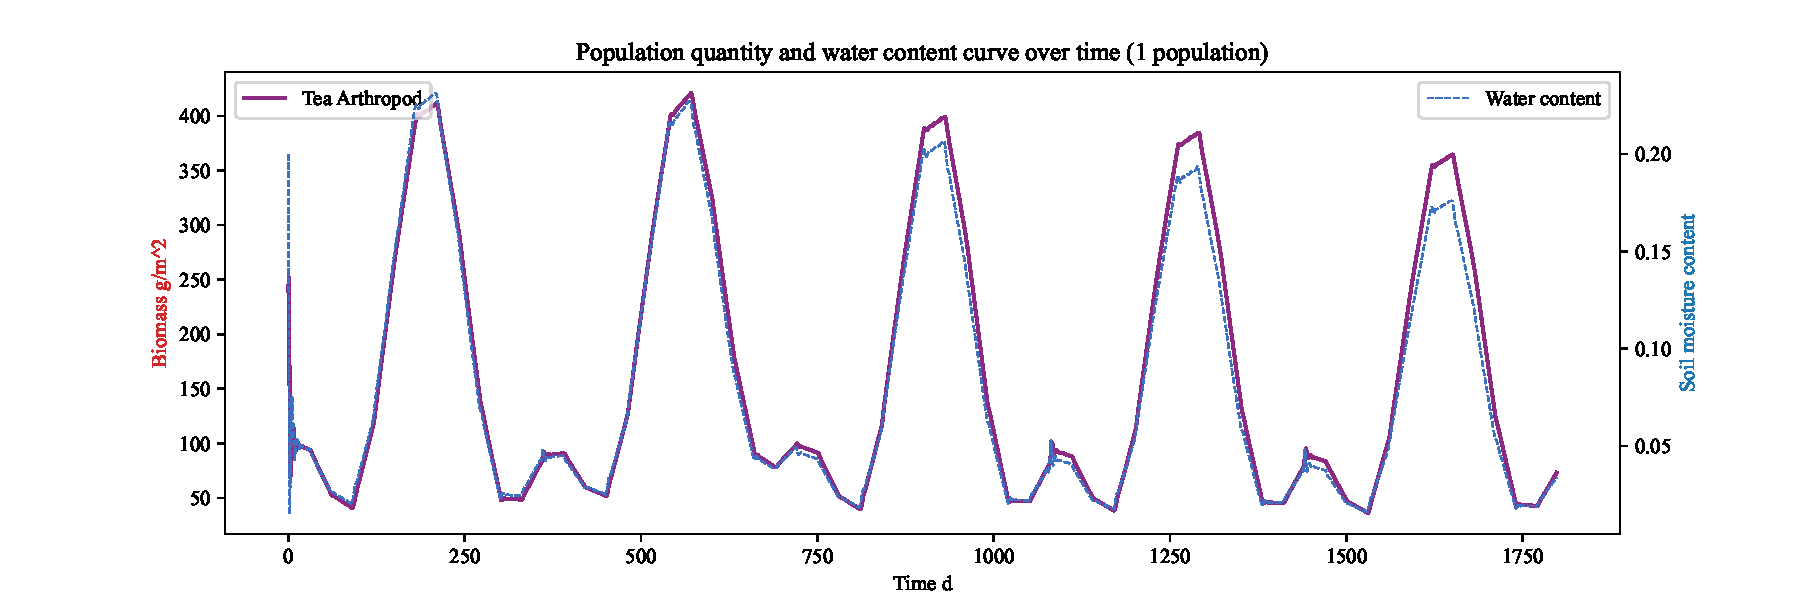
\includegraphics[width=\textwidth]{img/1_pure.pdf}
\end{subfigure}
\caption{Population quantity and moisture content curve over time (1 population)}
\label{fig:pure_1}
\end{figure}

Figure \hyperref[fig:pure_7]{\textcolor{blue}{9}} shows the changes in the biomass of each plant population when seven species are present. We can see that the ecosystem reaches a stable state due to the increase in the number of species. The ecosystem's total biomass and the soil's fertility factor rise yearly. The growth of other non-dominant species is somewhat restricted, but none die out ultimately. This shows that the increase in the number of biological species is beneficial to increase the stability of the ecosystem.

\begin{figure}[h] 
\centering 
\begin{subfigure}{ \textwidth}
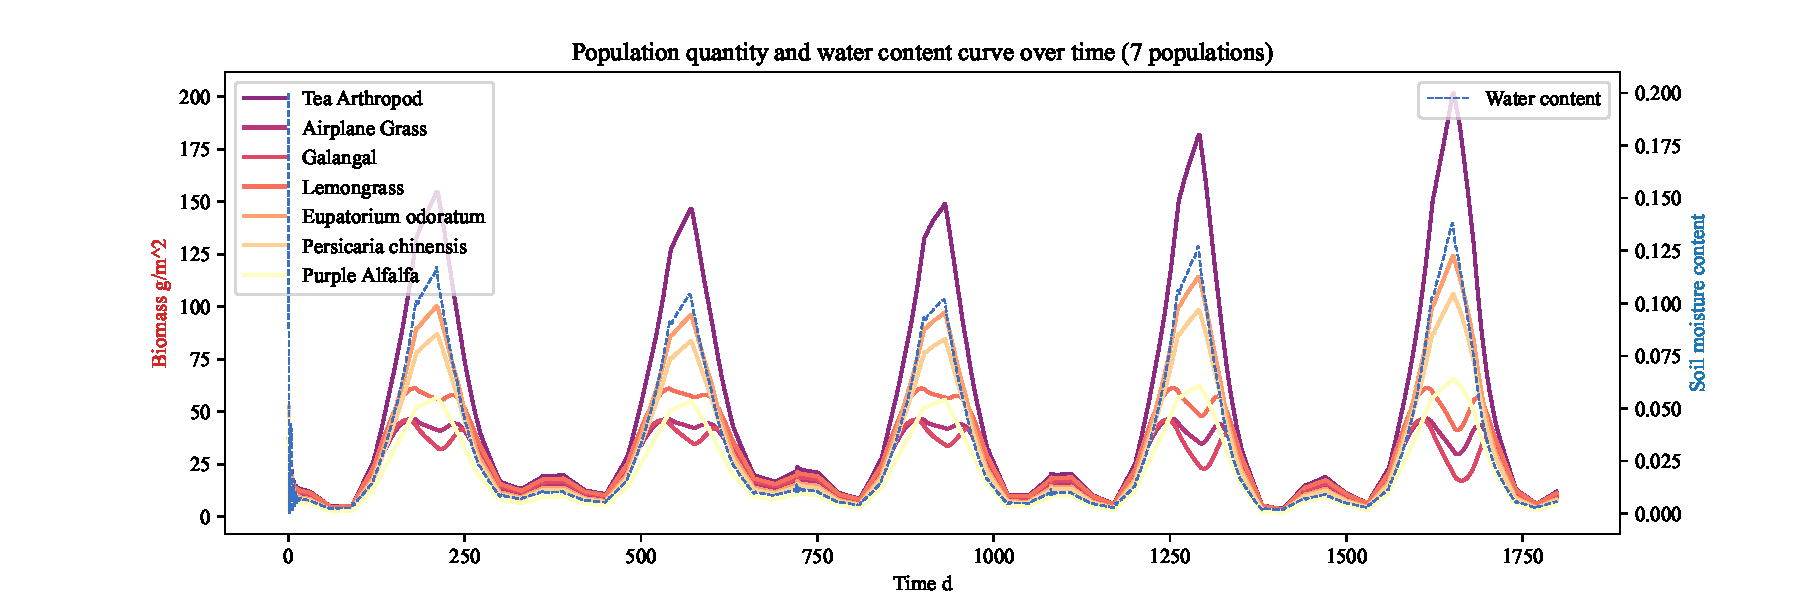
\includegraphics[width=\textwidth]{img/7_pure.pdf}
\end{subfigure}
\caption{Population quantity and moisture content curve over time (7 populations)}
\label{fig:pure_7}
\end{figure}


\subsection{Evaluation of Biodiversity}

\indent

Since the various functional components of the ecosystem are not fully considered in our model, we do not use the functional diversity index but take the Shannon index to measure the localized biodiversity, which is generally used as a fundamental measure of biodiversity. In our model, the calculation formula is as follows:


\begin{equation}
H=-\sum_ip_i \log_2\left(p_i \right),p_i=\frac{r_i(t)}{\sum_j r_j(t)}\
\end{equation}

Based on the calculation results in the previous section, we can obtain a trend of the average Shannon index in the presence of a different number of plant species. The results are shown in Figure \hyperref[fig:Shannon]{\textcolor{blue}{10}}:

\begin{figure}[h]
\centering 
\begin{subfigure}{ 0.45\textwidth}
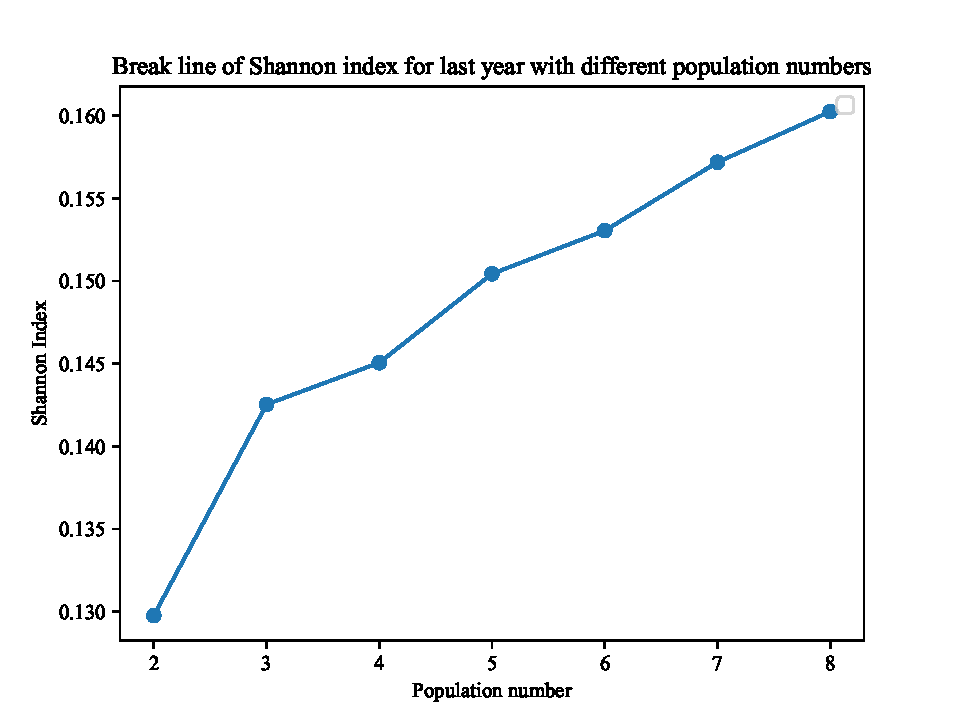
\includegraphics[width=\textwidth]{img/Shannon.pdf}
\end{subfigure}
\caption{Break line of Shannon index for last year with different population numbers)}
\label{fig:Shannon}
\end{figure}

The figure indicates that the Shannon index is increasing as the number of species increases. This is also consistent with the model predictions for species diversity.

\section{Sensitive Analysis}
\subsection{Drought Adaptability under Different Conditions}

\subsubsection{Methods for Changing Different Influencing Factors}

\indent

For drought severity, we observe the drought years 1977-1980 in the historical record and find that the precipitation in the drought years was about 80-90\% of the average years, so we adjust the precipitation in the drought years to 80\%, 85\%, 90\%, and 95\% of the average values to simulate different drought intensities and observe the impact on the plant community. 

For the drought frequency, since the time range of our study is $5$ years, we consider the effect of two types of drought frequencies: once every $2$ years and once every $3$ years. We change the drought frequency by changing the year the drought is applied. We apply drought in the second and fourth years to simulate biennial frequency. When simulating triennial frequency, we apply drought in the second year.

For species diversity, we change it by varying the number of plant species involved in the simulation.

\subsubsection{The Impact of Drought Frequency and Severity}

\indent

Figure \hyperref[fig:5_2_85]{\textcolor{blue}{11}} shows the change curves of species biomass versus soil moisture content when precipitation is adjusted to 85\%, drought frequency is once every $2$ years, and the number of species is 5. As can be seen from the graph, the first drought has a noticeable impact on the ecosystem, and the relative advantage of plants with greater reproductive capacity but weaker water absorption ability is significantly reduced. The ecosystem gradually declines over time, and it can be predicted that after a more extended period of evolution, this ecosystem will eventually go to degradation. Below we use this set of conditions as a baseline to discuss the effects of various factors on the ecosystem.

\begin{figure}[h]
\centering 
\begin{subfigure}{ 0.95\textwidth}
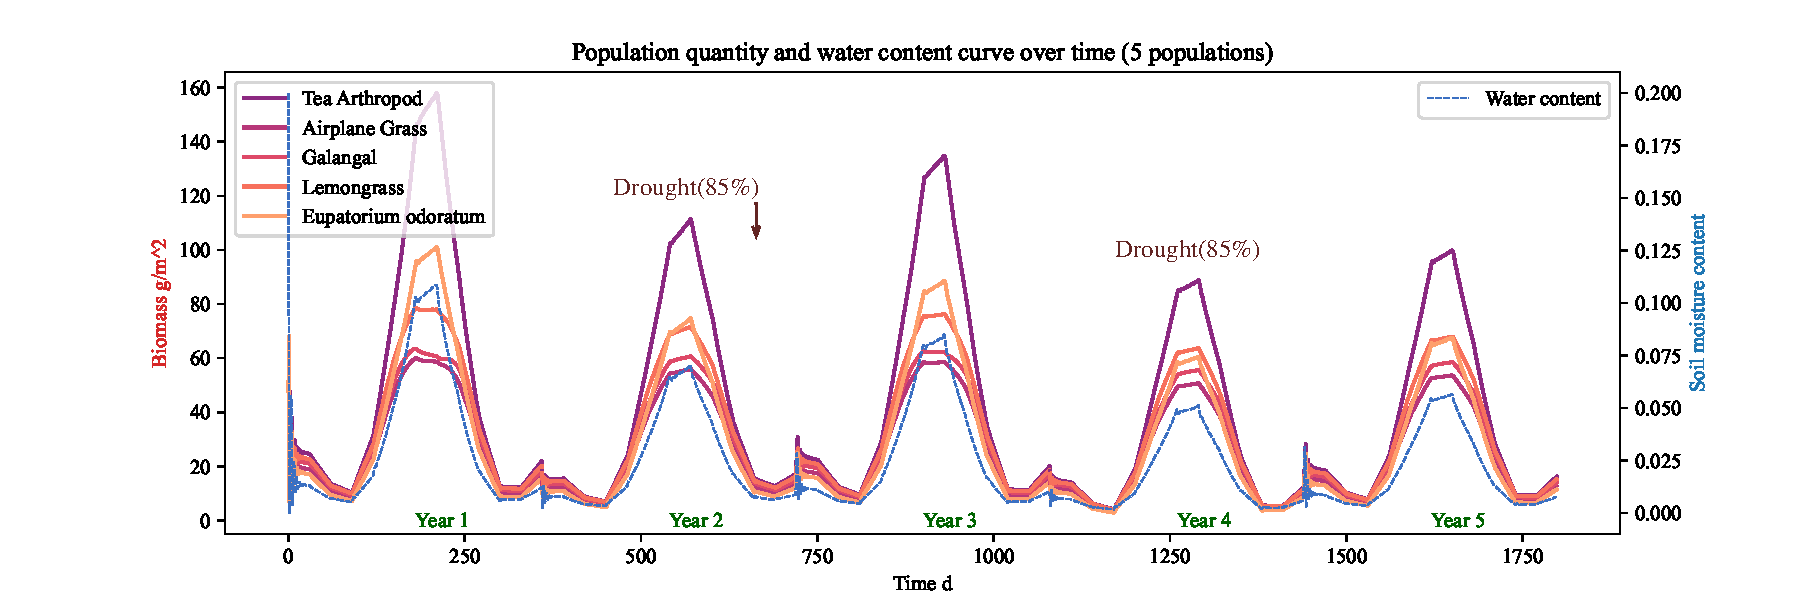
\includegraphics[width=\textwidth]{img/baseline_5_2_85.pdf}
\end{subfigure}
\caption{Population quantity and moisture content curve over time (5 populations), drought period $2$ years, precipitation rate 85\%}
\label{fig:5_2_85}
\end{figure}

Figure \hyperref[fig:5_1_85]{\textcolor{blue}{12}} shows the change curves of species biomass versus soil moisture content when both precipitation and the number of species stay the same, but the frequency of drought is reduced to once every $3$ years. The graph shows that the 3-year period has made the ecosystem return to the pre-drought level, so the ecosystem does not degrade. This indicates that drought frequency has a direct impact on whether the ecosystem can maintain a stable state or not. The higher the frequency of drought, the lower the likelihood that the ecosystem will maintain stability, which is also consistent with everyday experience.

\begin{figure}[h]
\centering 
\begin{subfigure}{ 0.95\textwidth}
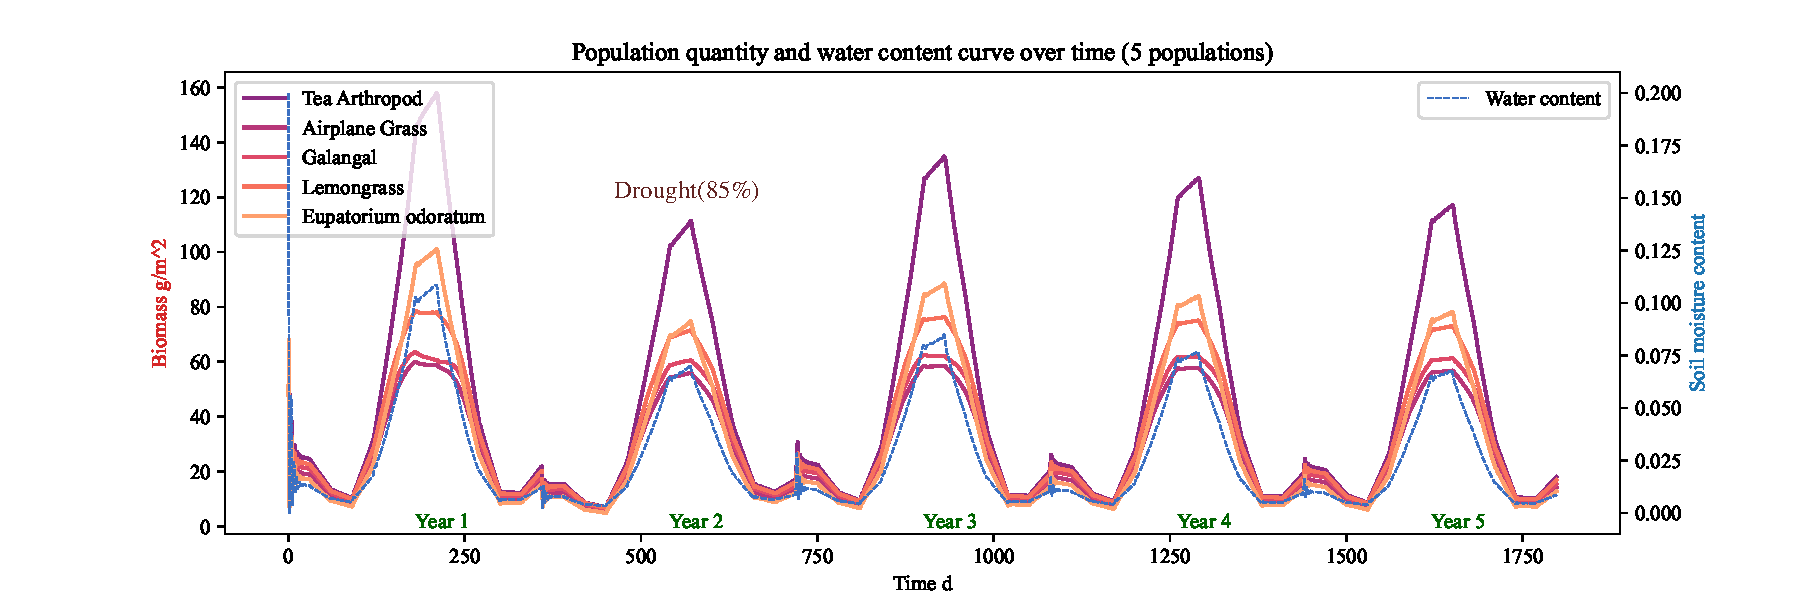
\includegraphics[width=\textwidth]{img/5_1_85.pdf}
\end{subfigure}
\caption{Population quantity and moisture content curve over time (5 populations), drought period $3$ years, precipitation rate 85\%}
\label{fig:5_1_85}
\end{figure}

Figure \hyperref[fig:5_2_90]{\textcolor{blue}{13}} shows the curves when the frequency of drought and the number of species are the same as the baseline and the precipitation increases to 90\%. In this situation, we can see that drought's damage to the ecosystem is significantly weaker. This indicates that the greater the level of drought severity is, the more severe damage it brings to the ecosystem.

\begin{figure}[h]
\centering 
\begin{subfigure}{ 0.95\textwidth}
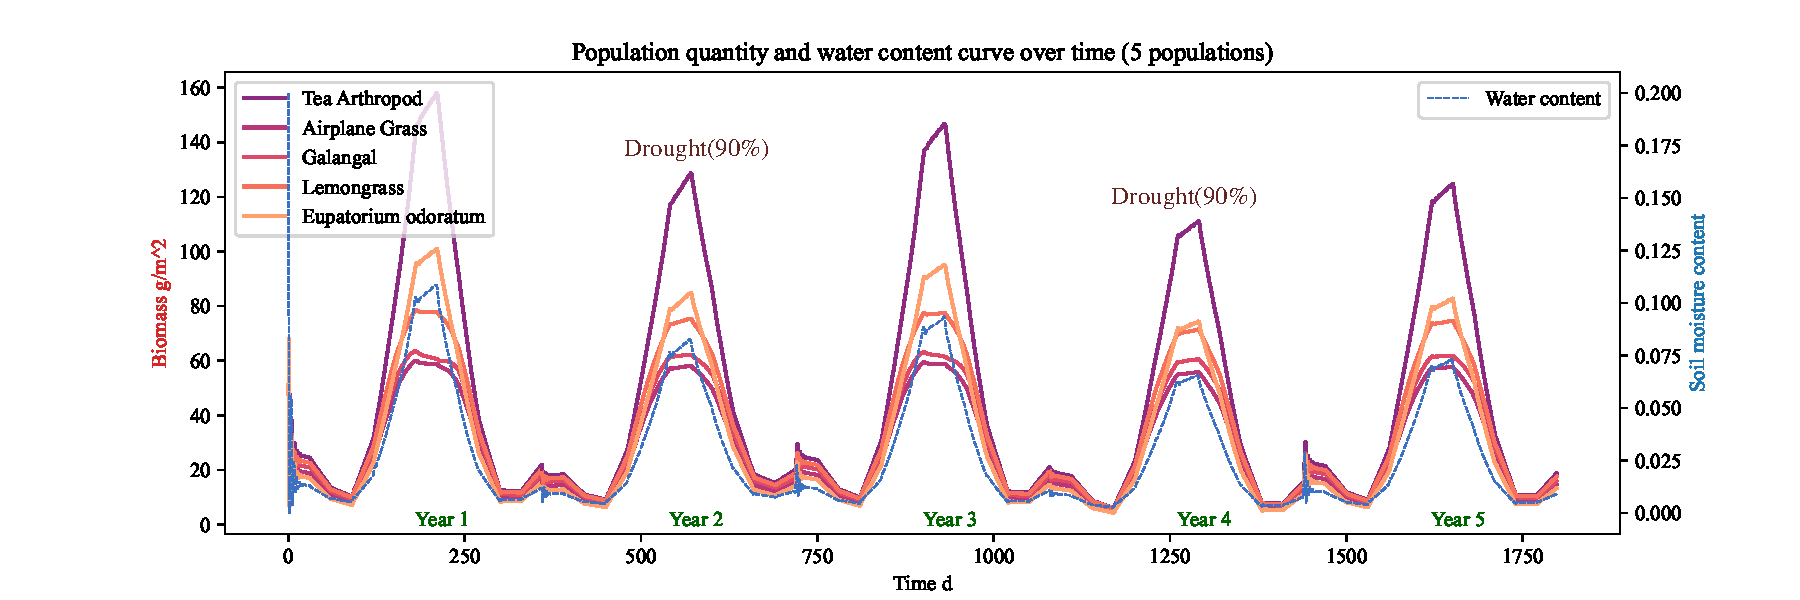
\includegraphics[width=\textwidth]{img/5_2_90.pdf}
\end{subfigure}
\caption{Population quantity and moisture content curve over time (5 populations), drought period 2 years, precipitation rate 90\%}
\label{fig:5_2_90}
\end{figure}

\subsubsection{The Impact of Localized Biodiversity}

\indent

Figure \hyperref[fig:7_2_85]{\textcolor{blue}{14}} shows the variation of biomass versus soil moisture content when the number of species in the baseline is changed to 7 and other conditions remain unchanged. It can be seen that the effect of the same severity of drought with 7 species is significantly less than the situation with 5 species, indicating that the drought adaptability of the ecosystem is significantly enhanced.

\begin{figure}[h]
\centering 
\begin{subfigure}{ 0.95\textwidth}
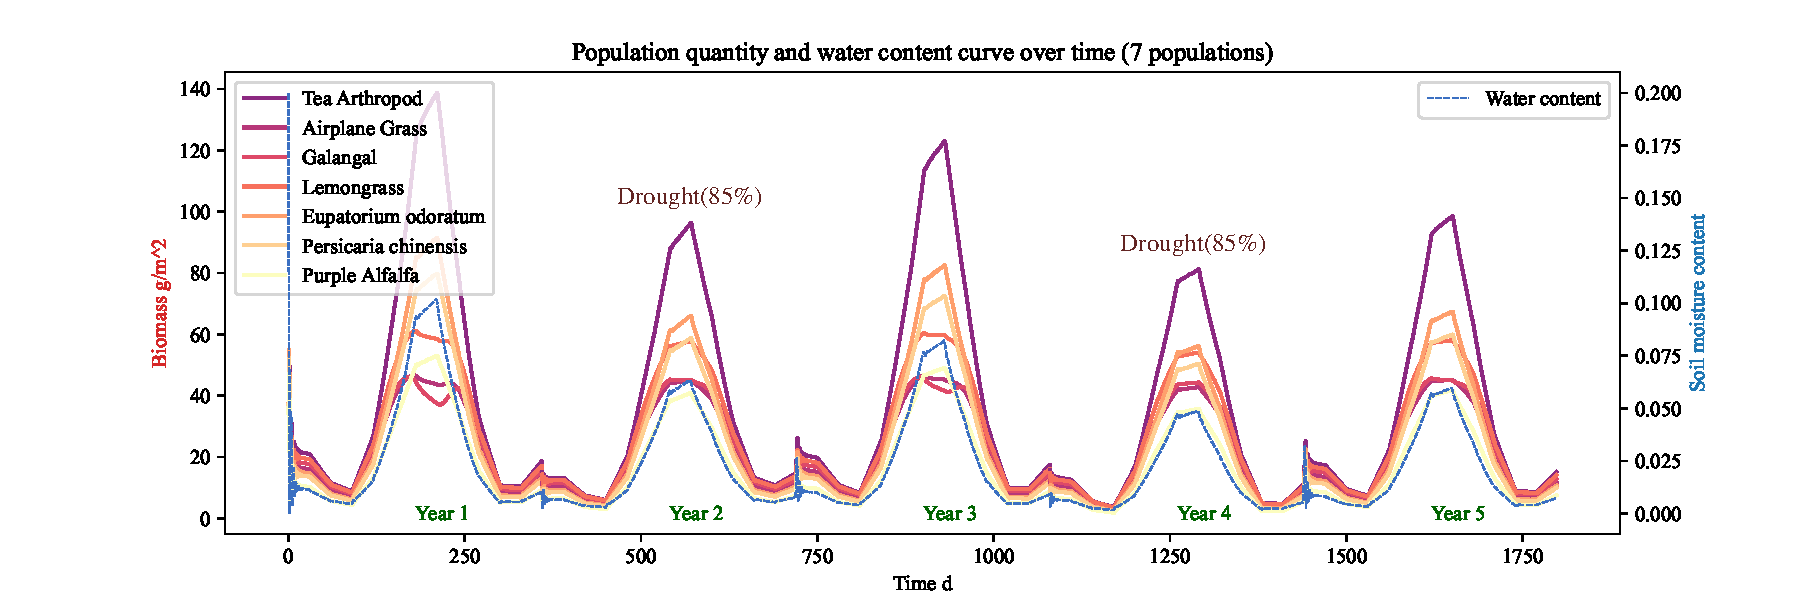
\includegraphics[width=\textwidth]{img/7_2_85.pdf}
\end{subfigure}
\caption{Population quantity and moisture content curve over time (7 populations), drought period $2$ years, precipitation rate 85\%}
\label{fig:7_2_85}
\end{figure}

Figure \hyperref[fig:3_2_85]{\textcolor{blue}{15}} shows the curves when the number of species in the baseline is changed to 3 and other conditions remain unchanged. It can be seen that the effect of the same severity of drought with 7 species is more significant than the situation with 5 species, indicating that the drought adaptability of the ecosystem is significantly weakened.

\begin{figure}[h]
\centering 
\begin{subfigure}{ 0.92\textwidth}
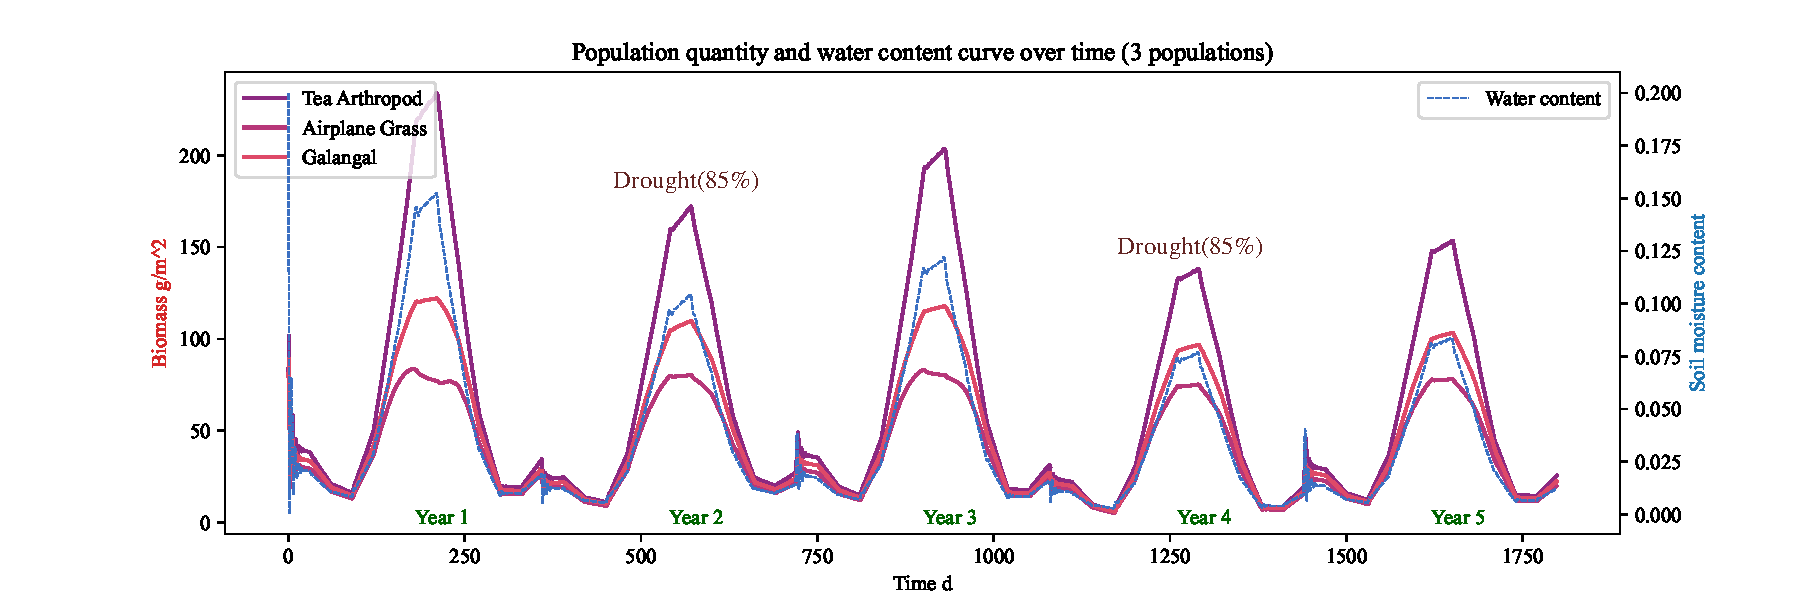
\includegraphics[width=\textwidth]{img/3_2_85.pdf}
\end{subfigure}
\caption{Population quantity and moisture content curve over time (3 populations), drought period 2 years, precipitation rate 85\%}
\label{fig:3_2_85}
\end{figure}



\subsubsection{Conclusion}

\indent

By repeating the above analysis steps, we can derive a contour plot of the fertility factor of the ecosystem in year 5 under different drought frequencies and levels of severity. The bigger the fertility factor in the 5th year, the better the ecosystem recovers its function under given conditions. We can learn from the above graphs that the more species present in a plant community, the better the community's ability to adapt to drought.


\begin{figure}
  \centering
  \hspace{1cm}
  \begin{subfigure}{0.4\textwidth}
    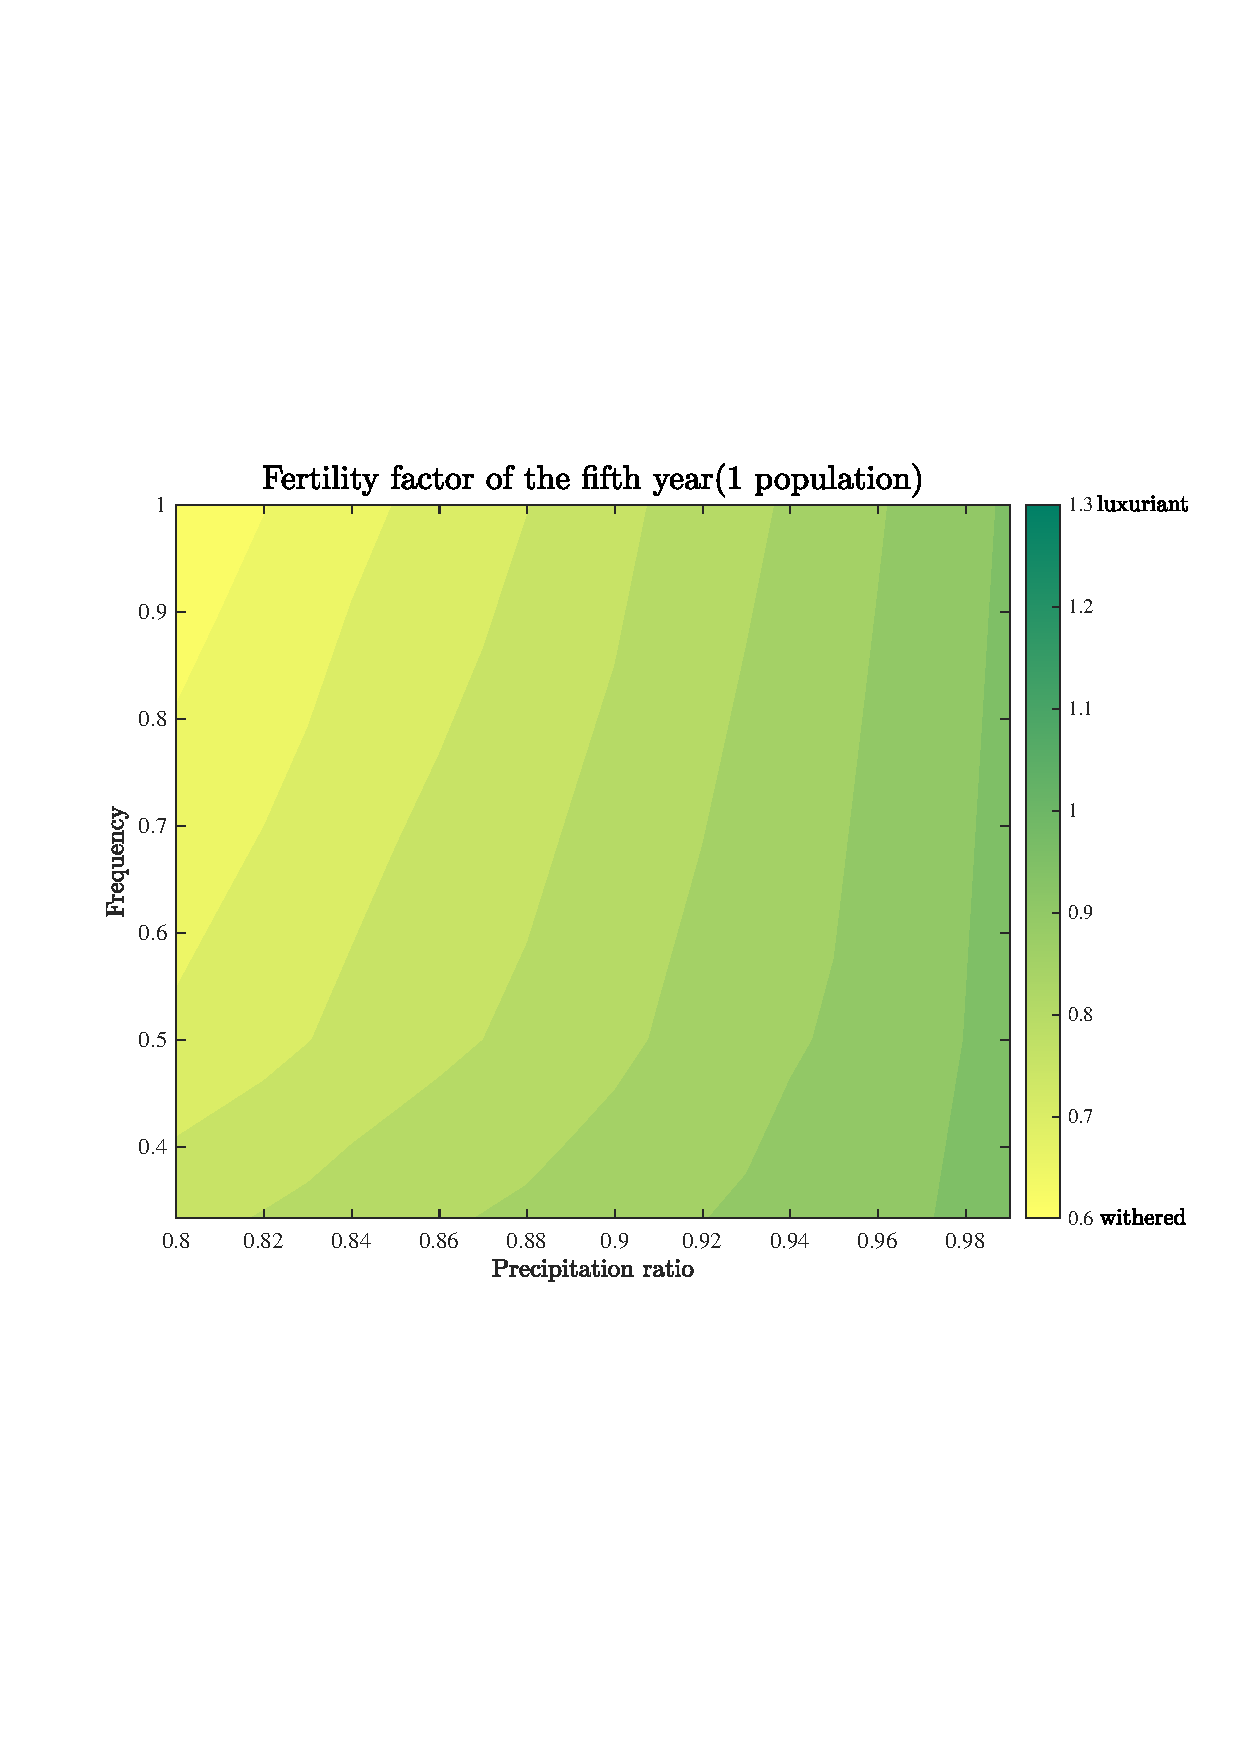
\includegraphics[width=5.6cm]{img/Contour_1.pdf}
    \caption{Population number: 1$\quad\quad\quad$}
    \label{fig:Population number 1}
  \end{subfigure}
  \hspace{0cm}
  \begin{subfigure}{0.4\textwidth}
    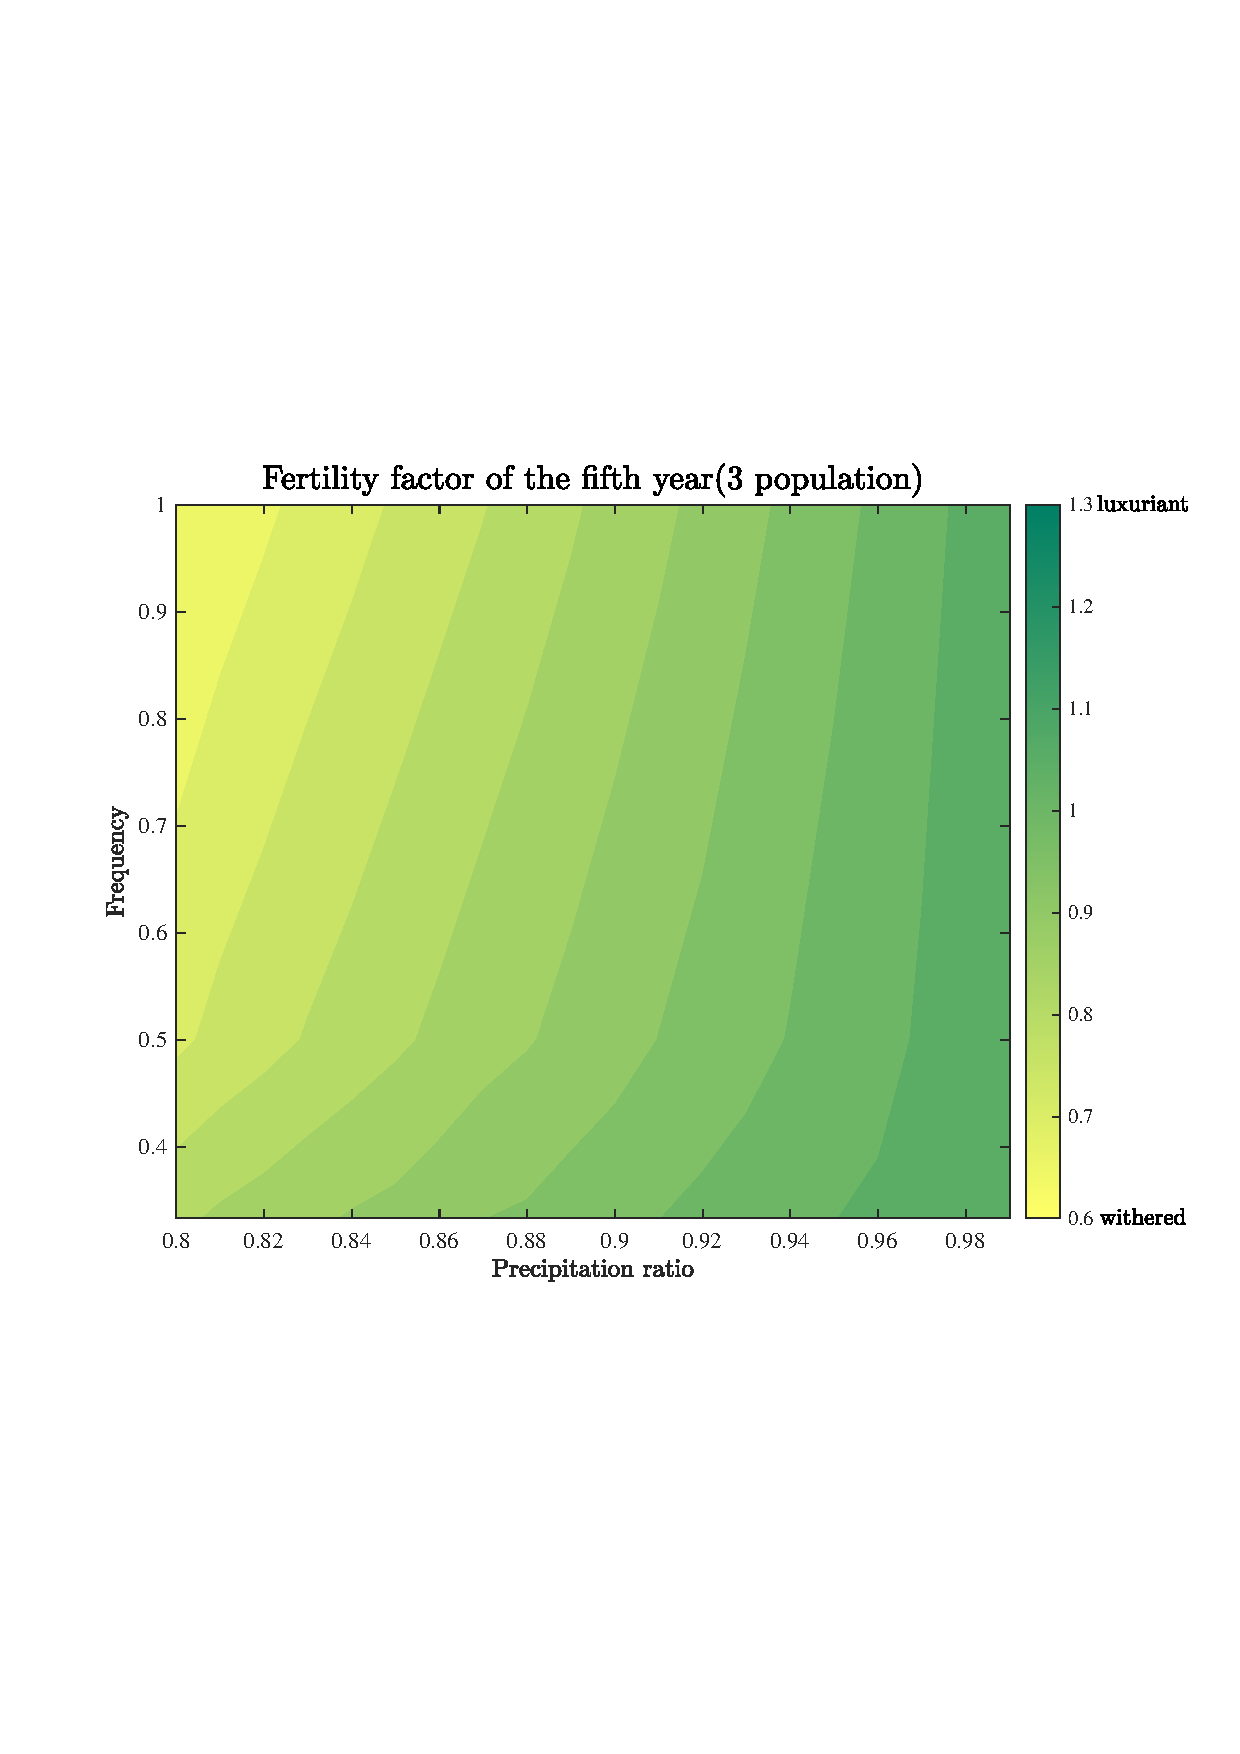
\includegraphics[width=5.8cm]{img/Contour_3.pdf}
    \caption{Population number: 3$\quad\quad\quad$}
    \label{fig:Population number 3}
  \end{subfigure}
  
  \hspace{1.1cm}
  \begin{subfigure}{0.4\textwidth}
    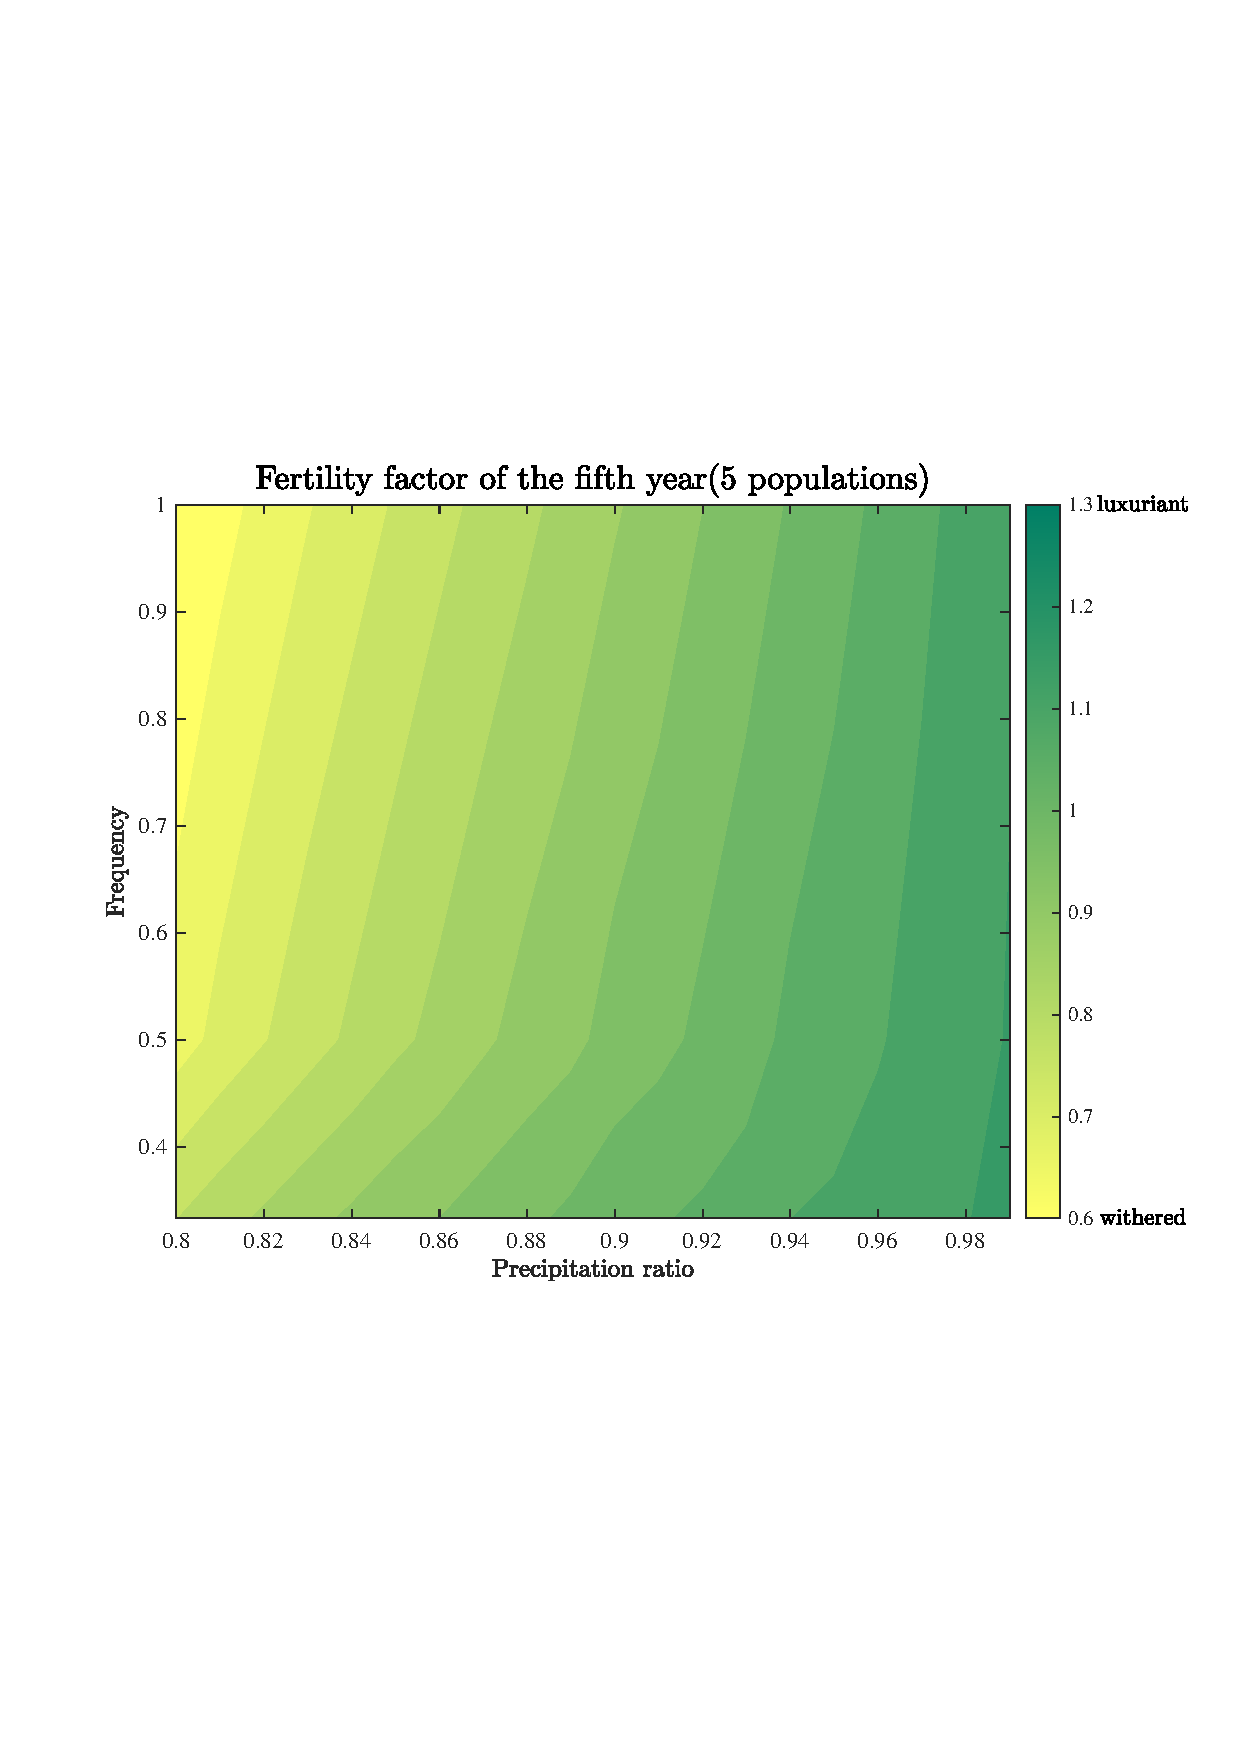
\includegraphics[width=5.6cm]{img/Contour_5.pdf}
    \caption{Population number: 5$\quad\quad\quad$}
    \label{fig:subfigure3}
  \end{subfigure}
  \hspace{0cm}
  \begin{subfigure}{0.4\textwidth}
    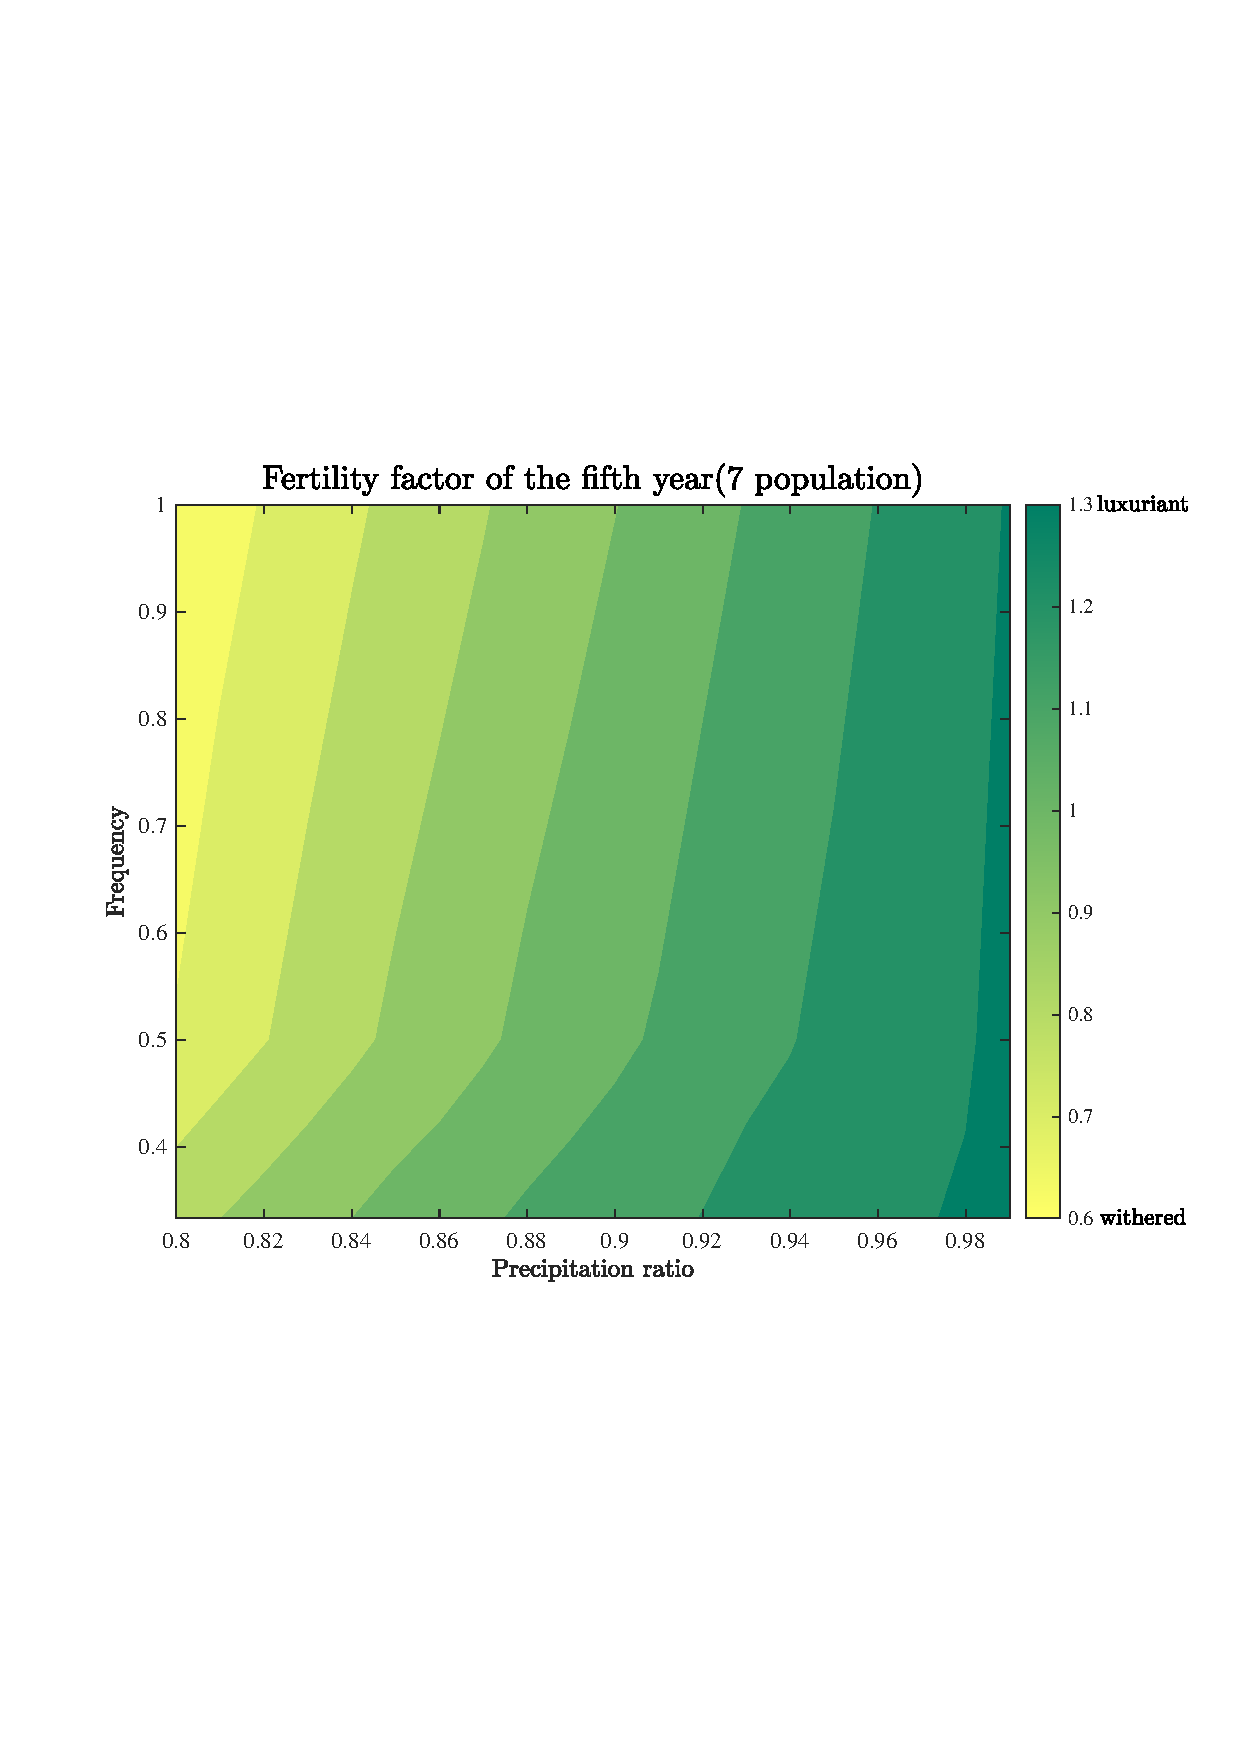
\includegraphics[width=5.7cm]{img/Contour_7.pdf}
    \caption{Population number: 7$\quad\quad\quad$}
    \label{fig:subfigure4}
  \end{subfigure}
  \caption{The relationship between soil fertility factor and drought frequency and precipitation rate under different biological population conditions}
  \label{fig:Contours}
\end{figure}




\subsection{The Impact of Environmental Capacity K(t)}

\indent

The choice of coefficient for the environmental holding capacity $K(t)$ in our model is artificial, while the environmental size is positively correlated with the environmental holding capacity. Therefore we simulate different environment sizes by modifying the coefficient of $K(t)$. A larger coefficient represents a larger environment. The following two figures show the results without changing the coefficient of $K(t)$ and after increasing the coefficient of $K(t)$, respectively.


\begin{figure}[h]
\centering 
\begin{subfigure}{ \textwidth}
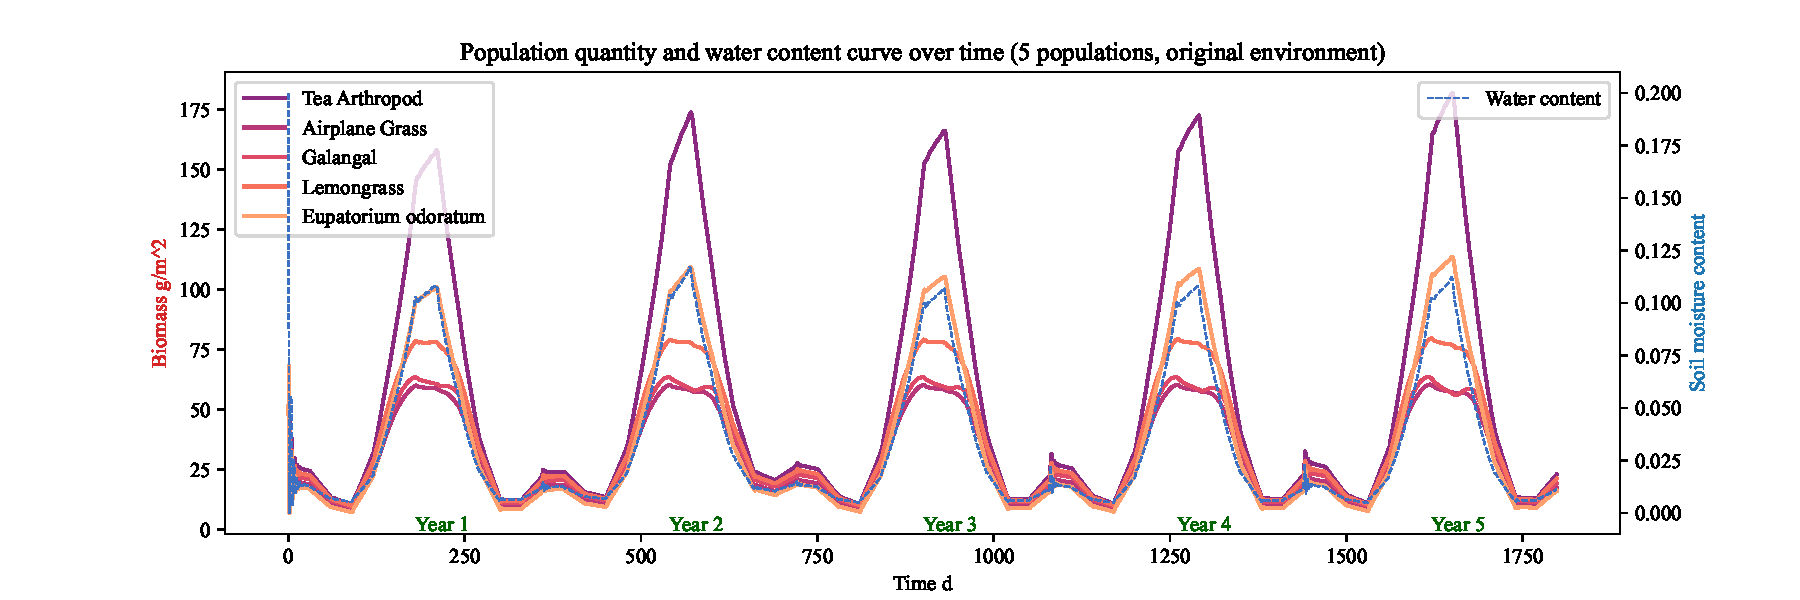
\includegraphics[width=\textwidth]{img/origin_K_5.pdf}
\end{subfigure}
\caption{Population quantity and moisture content curve over time (5 populations, original environment)}
\label{fig:origin_K_5}
\end{figure}


\begin{figure}[h]
\centering 
\begin{subfigure}{ \textwidth}
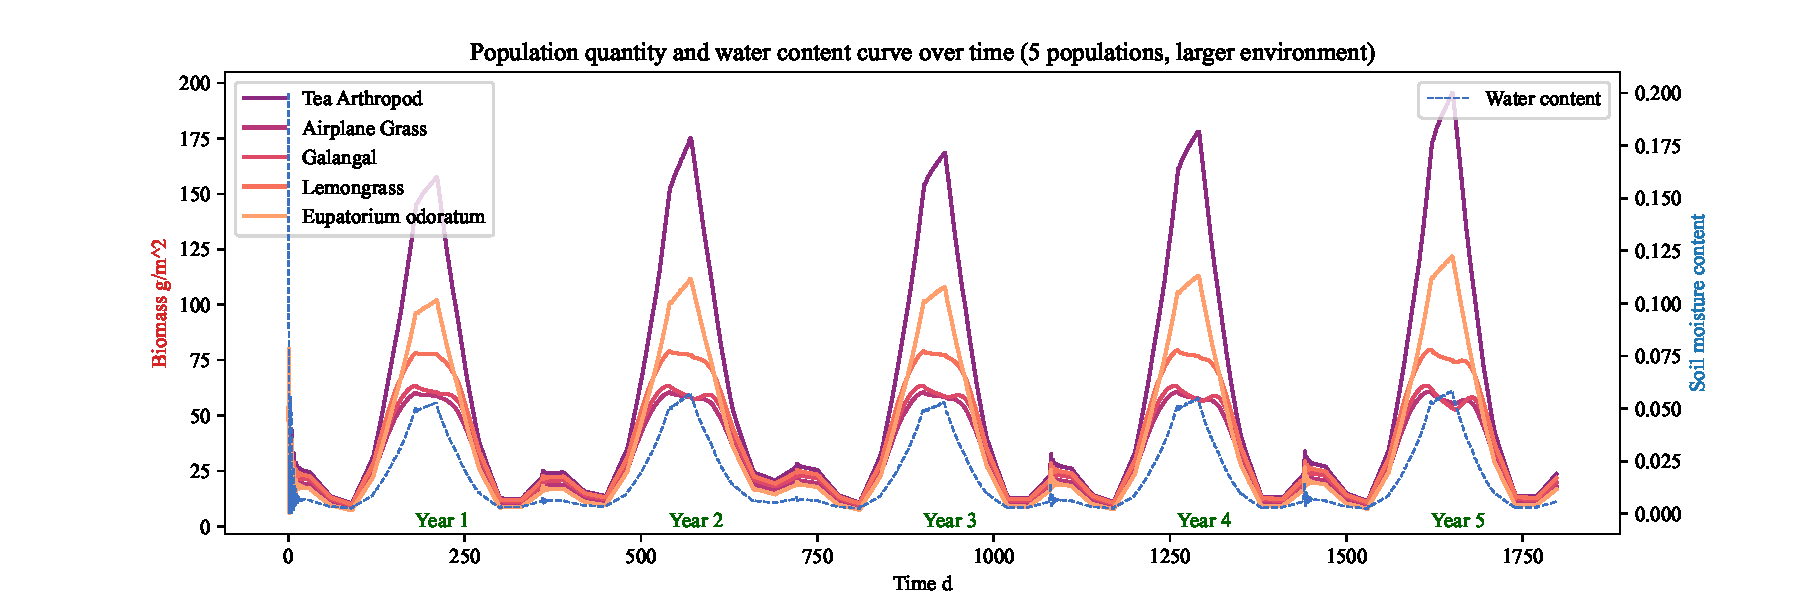
\includegraphics[width=\textwidth]{img/larger_K_5.pdf}
\end{subfigure}
\caption{Population quantity and moisture content curve over time (5 populations, larger environment)}
\label{fig:larger_K_5}
\end{figure}

We can see a slight increase in biomass in the environment, but the general conclusions of the model do not change. This indicates that the general conclusions of the model do not change significantly within a specific range of environmental size.

\subsection{The Impact of Pollution}

\indent

Pollution can degrade the local ecology and lead to the death of a large number of plants in a short period. Therefore, we take the approach of reducing the biomass growth rate in a short period in our model to simulate the effects of pollution. We impose the effects of pollution lasting about three months in this model, and the results are as follows:

\begin{figure}[h]
\centering 
\begin{subfigure}{ \textwidth}
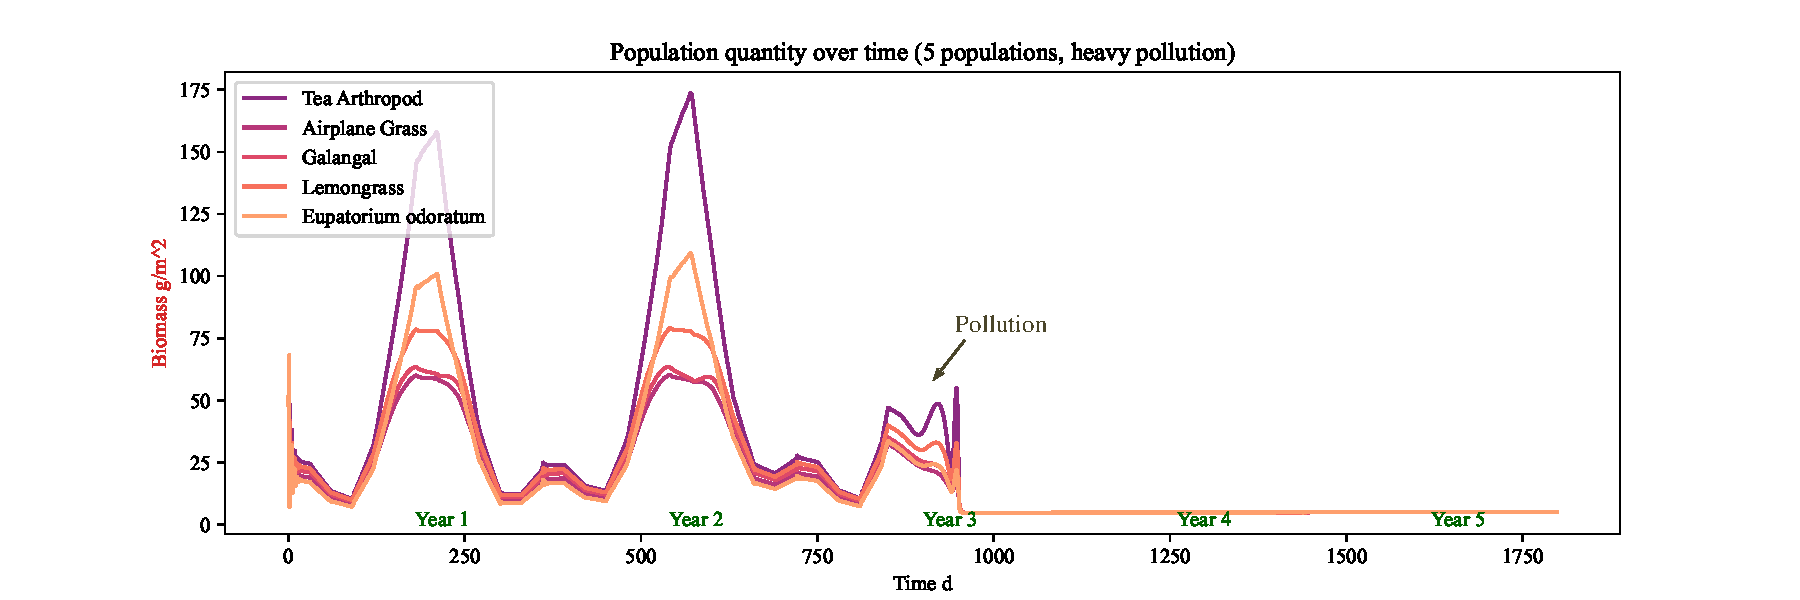
\includegraphics[width=\textwidth]{img/pollution.pdf}
\end{subfigure}
\caption{Population quantity over time (5 populations, heavy pollution)}
\label{fig:pollution}
\end{figure}

\subsection{The Impact of the Types of Species}

\indent

By selecting five other plants without changing the baseline conditions, we can obtain a new variation curve. The results are as follows:

\begin{figure}[h]
\centering 
\begin{subfigure}{ \textwidth}
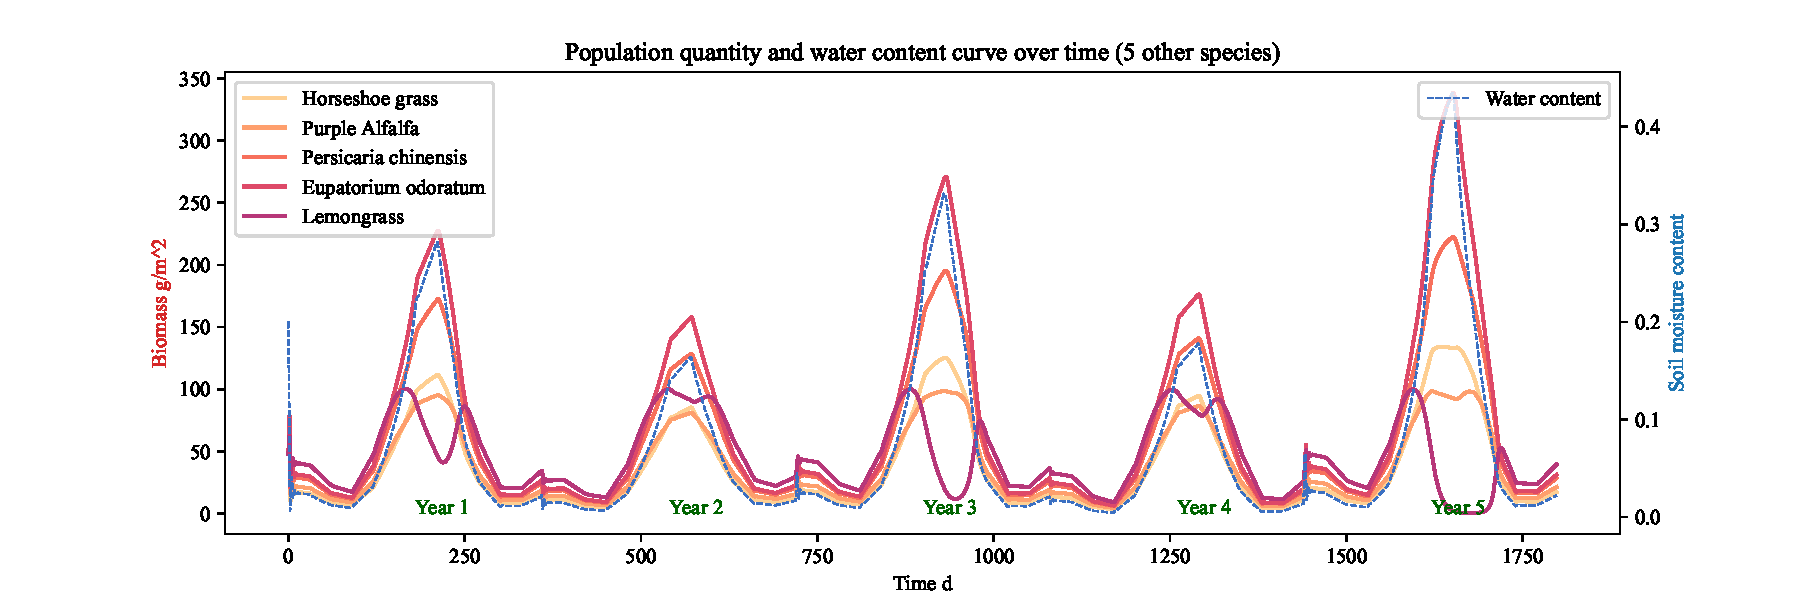
\includegraphics[width=\textwidth]{img/other_5_2_85.pdf}
\end{subfigure}
\caption{Population quantity and moisture content curve over time (5 other species)}
\label{fig:other_5_2_85}
\end{figure}

As we can see from the graph, the competitive relationship between species changes. And the community is better able to recover from drought. If you replace selected species with other species, the competition between species and the resilience of the entire ecosystem will also change, but there is no clear pattern of change. Such changes are significantly related to the species' ability to absorb water, reproduce and survive. This suggests that introducing the right mix of species into an ecosystem can maximize the benefits of the entire ecosystem.

To explore the impact of the number of biological species on the drought resistance of an ecosystem, we change the number of biological species under different environmental conditions and investigate the value of soil fertility factors in the fifth year. The resulting data line graph is shown below:

\begin{figure}[h]
\centering 
\begin{subfigure}{ 0.5\textwidth}
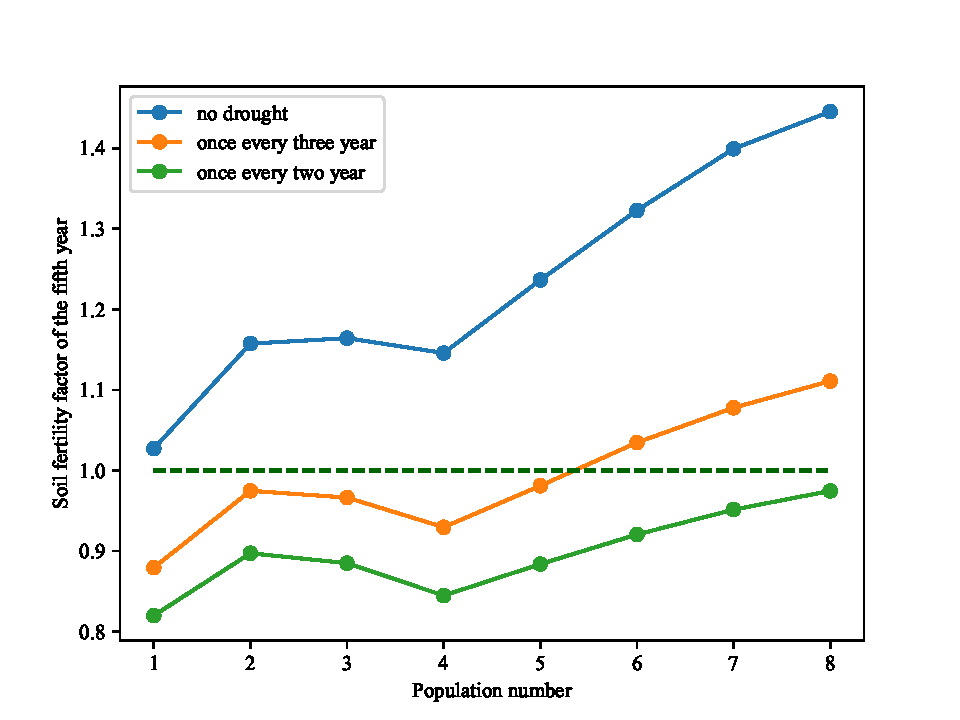
\includegraphics[width=\textwidth]{img/final.pdf}
\end{subfigure}
\caption{Changes in the number of plant species in the fifth year of fertility factor under standard drought conditions}
\label{fig:final}
\end{figure}

From the graph, it can be seen that when the number of species is less than 4, the drought resistance of the ecosystem fluctuates within a specific range and does not improve significantly. When the number of species exceeds 4, the more species there are, the stronger the drought resistance of the ecosystem becomes. Therefore, at least 4 species are needed for significant improvement, and this improvement has a roughly linear relationship within the scope of the study. At the same time, the higher the frequency of drought, the weaker the improvement, which also indicates that the stability of the ecosystem is limited.

\section{Conclusions}

\subsection{Strengths and Weaknesses}
\textbf{Strengths:}
\indent

\textbf{Reliable data sources:} The model selects the climate historical data of nearly a century in New Mexico from the website of the National Meteorological Bureau of the United States, and performs fitting. Multiple academic papers on the study of grassland plants have been refered to, making the data source of the model convincing.

\textbf{Innovative and diverse modeling tools:} The model integrates various evaluative and analytical modeling methods, establishes differential equation models, and adopts AHP and FEA solutions. Both the modeling and solving methods reflect innovation and diversity.

\textbf{Clear logic and well-defined hierarchy:} We first build a Selection model to simulate the genetic evolution as well as a Competition model to understand interspecific competition. Then we integrate the results from these two models to obtain an Interactive model of bio-ecological interaction. After that, functions are added and modifications are made, resulting in a clear and logical overall structure.

\textbf{Comprehensive consideration of multiple factors:} The article comprehensively considers the impact of various factors when modeling, including the evolutionary trends, the competition among populations, the interaction between biology and the environment, and the influence of abnormal factors such as irregular drought and pollution, demonstrating a comprehensive approach to the problem.


\noindent
\textbf{Weaknesses:}

\textbf{Not considering the influence of other factors in the ecosystem:} The article mainly focuses on the interaction between plants and the environment without fully considering the impact of animals and some non-natural factors.

\textbf{Limited species and period of the study:} Due to the inability to conduct field investigations, we only study eight species and could not conduct in-depth research on more plants. At the same time, due to limitations in computing equipment, we could not simulate the evolutionary trends over a more extended period.

\subsection{Suggestions}

\indent

Based on our SCI-E model, we propose several suggestions to ensure the long-term viability of a plant community:


\begin{itemize}
\item \textbf{Improving and maintaining localized biodiversity in plant communities.}

Biodiversity is an important influencing factor in the health and adaptability of plant communities. Diverse plant communities are better adapted to changing environmental conditions, such as drought and high heat. To improve and maintain localized biodiversity, it may be necessary to take actions such as removing invasive species and planting suitable plants.
 
 \item \textbf{Selecting appropriate plant combinations. }

Plant combinations are important because certain species can have positive or negative effects on one another. Selecting appropriate plant combinations can help support the health and growth of individual plants and the community. Factors to consider when selecting plant combinations include plant species diversity, water, and nutrient requirements, the presence of companion species, etc.
 
 
\item \textbf{Minimizing pollution and other ecologically destructive human factors.}

Ecologically destructive human factors can significantly impact plant communities, leading to declines in plant health and reduced biodiversity. Other human factors, such as habitat fragmentation and invasive species, can negatively impact plant communities. Minimizing these factors by implementing sustainable land use practices, reducing emissions, and other methods can help support plant communities' long-term viability.

\end{itemize}

 Overall, these actions can help create a more resilient and diverse plant community, which can support the health and well-being of a plant community and the larger environment.

\newpage
\begin{thebibliography}{99}
\addcontentsline{toc}{section}{Reference}

\bibitem{1} \url{https://image.baidu.com/}
\bibitem{2} \url{https://charts.climate.lsu.edu/trends}
\bibitem{3} Kumar, M., Kumar, V., Prasad, S. M., \& Prasad, R. (2017). Differential response of three grass species to drought stress: Effect on biomass accumulation, leaf water content, and gas exchange. Journal of Plant Interactions, 12(1), 437-447.
\bibitem{4} Song, C., Jin, Y., Sun, Y., Wang, J., Zhang, Y., Guan, Y., ... \& Han, L. (2018). The physiological and biochemical responses of four grass species to drought stress in northern China. PeerJ, 6, e5443.
\bibitem{5} Sperry, J. S., Meinzer, F. C., \& McCulloh, K. A. (2008). Safety and efficiency conflicts in hydraulic architecture: scaling from tissues to trees. Plant, cell \& Environment, 31(4), 632-645.
\bibitem{6} Brevik, E. C., \& Cerdà, A. (2018). The interdisciplinary nature of the soil. Soil, 4(1), 1-4.
\bibitem{7} Maestre, F. T., Castillo-Monroy, A. P., Bowker, M. A., Ochoa-Hueso, R., \& Gallardo, A. (2012). Species richness effects on ecosystem multifunctionality depend on evenness, composition, and spatial pattern. Journal of Ecology, 100(2), 317-330.
\bibitem{8}  Marra, D. M., Chambers, J. Q., Higuchi, N., Trumbore, S. E., Ribeiro, G. H. P. M., Santos, J. d., \& Nóbrega, G. N. (2010). Effects of soil water content on soil respiration in forests and cattle pastures of eastern Amazonia. Biogeochemistry, 105(1), 119-129.

\end{thebibliography}

\newpage

\begin{appendices}
\setstretch{1}
Note: We only attach the core code in the SCI-E model.

\noindent \textbf{\textcolor[rgb]{0.353,0.753,0.612}{Python source for Population iterative simulations (Figure \hyperref[fig:5_2_85]{\textcolor{blue}{11}}\textcolor{blue}{-}\hyperref[fig:3_2_85]{\textcolor{blue}{15}})}}
\lstinputlisting[language=Python]{./code/differential_equations.py}
\textbf{\textcolor[rgb]{0.353,0.753,0.612}{Matlab source for Contour maps (Figure \hyperref[fig:Contours]{\textcolor{blue}{16}}) }}
\lstinputlisting[language=Matlab]{./code/surface_three.m}

\end{appendices}
\end{document}